\documentclass[global,twocolumn]{svjour}
\usepackage{cite}
\usepackage{amsmath}
\usepackage{amsfonts}
\usepackage{url}
\usepackage{comment}
\usepackage{paralist}
\usepackage{graphicx}
\graphicspath{{./figs/}}
\usepackage{listings}
\usepackage[usenames,dvipsnames,svgnames,table]{xcolor}
\usepackage{flushend}
\usepackage{hyperref}
\usepackage[firstpage]{draftwatermark}
\usepackage[lighttt]{lmodern}
\usepackage[normalem]{ulem}

\definecolor{dkgreen}{rgb}{0,0.6,0}
\definecolor{mauve}{rgb}{0.58,0,0.82}
\definecolor{light-gray}{gray}{0.88}

\lstdefinestyle{myML}
{frame=none,
  basicstyle=\ttfamily,
  language=ML,
  aboveskip=3mm,
  belowskip=3mm,
  showstringspaces=false,
  columns=flexible,
  numbers=none,
  numberstyle=\tiny\color{gray},
  commentstyle=\color{dkgreen},
  stringstyle=\color{mauve},
  breaklines=false,
  breakatwhitespace=true,
  tabsize=2,
  linewidth=2\linewidth
}

\lstdefinestyle{agree}
{frame=none,
  basicstyle=\ttfamily,
  language=ML,
  aboveskip=3mm,
  belowskip=3mm,
  showstringspaces=false,
  columns=flexible,
  numbers=none,
  numberstyle=\tiny\color{gray},
  commentstyle=\color{dkgreen},
  stringstyle=\color{mauve},
  breaklines=false,
  breakatwhitespace=true,
  tabsize=2,
  linewidth=2\linewidth,
  morecomment=[l]{--},
  escapeinside={*}{*},
  morekeywords={eq, bool, guarantee, assume, true, false, pre, not, and, or, property, const, Historically, Since, Once, event, annex, Implementation, process, subcomponents}
}

\hyphenation{op-tical net-works semi-conduc-tor Cake-ML}

% Comment macros
\newcommand{\newjunk}[1]{\textcolor{red}{#1}}
\newcommand{\oldjunk}[1]{\sout{#1}}

\newcommand{\konst}[1]{\ensuremath{\mathsf{#1}}}
\newcommand{\imp}{\Rightarrow}
\newcommand{\set}[1]{\ensuremath{\{ {#1} \}}}
\newcommand{\sem}[1]{\ensuremath{[\![ #1 ]\!]}}
\newcommand{\kstar}[1]{\ensuremath{{#1}^{*}}}
\newcommand{\Lang}[1]{\ensuremath{{\mathcal L}({#1})}}
\newcommand{\Eqs}{\ensuremath{\mathit{Eqs}}}
\newcommand{\itelse}[3]{\mbox{$\mathtt{if}\ {#1}\ \mathtt{then}\ {#2}\ \mathtt{else}\ {#3}$}}

\newcommand{\figref}[1]{Fig.~\ref{#1}}
\newcommand{\secref}[1]{Sec.~\ref{#1}}
\newcommand{\lineref}[1]{Line~\ref{#1}}
\newcommand{\linesref}[2]{Lines~\ref{#1}--\ref{#2}}

% Acronym macros
\newcommand{\brfcs}{BriefCASE}
\newcommand{\agr}{AGREE}
\newcommand{\splt}{SPLAT}
\newcommand{\ckml}{CakeML}

\newcommand{\ie}{\textit{i.e.}}
\newcommand{\eg}{\textit{e.g.}}
\newcommand{\etal}{\textit{et al.}}
\newcommand{\etc}{\textit{etc.}}
\newcommand{\adhoc}{\textit{ad hoc}}

\journalname{Software and Systems Modeling}

\begin{document}
\title{
  Synthesizing Verified Components for Cyber Assured Systems Engineering
  \thanks{DISTRIBUTION STATEMENT A.  Approved for public release.}
}

\author{
  Eric Mercer\inst{1}    \and
  Konrad Slind\inst{2}   \and
  Isaac Amundson\inst{2} \and
  Darren Cofer\inst{2}   \and
  Junaid Babar\inst{3}   \and
  David Hardin\inst{3}
}

\institute{
  Brigham Young University        \\
  Provo, Utah                     \and
  Applied Research and Technology \\
  Collins Aerospace               \\
  Minneapolis, Minnesota          \and
  Applied Research and Technology \\
  Collins Aerospace               \\
  Cedar Rapids, Iowa
}

\date{Received: date / Revised version: date}

\maketitle

\begin{abstract}
Avionics need to be engineered to be cyber-resilient meaning that systems are able to detect and recover from attacks or safely shutdown.
%
As there are few development tools for cyber-resiliency, designers rely on guidelines and checklists, sometimes missing vulnerabilities until late in the process where remediation is expensive.
%
Our solution is a model-based approach with cyber-resilience-improving transforms that insert high-assurance components such as filters to block malicious data or monitors to detect and alarm anomalous behavior.
%
Novel is our use of model checking and a verified compiler to specify, verify, and synthesize these components.
%
We define \emph{code contracts} as formal specifications that designers write for high-assurance components, and \emph{test contracts} as tests to validate their behavior.
%
A model checker proves whether or not code contracts satisfy test contracts in an iterative development cycle.
%
The same model checker also proves whether or not a system with the inserted components, assuming they adhere to their code contracts, provide the desired cyber-resiliency for the system.
%
We define an algorithm to synthesize implementations for code contracts in a semantics-preserving way that is backed by a verified compiler.
%
The entire workflow is implemented as part of the open source \emph{\brfcs} toolkit.
%
We report on our experience using \brfcs\ with a case study on a UAV system that is transformed to be cyber-resilient to communication and supply chain cyber attacks.
%
Our case study demonstrates that writing code contracts and then synthesizing correct implementations from them is feasible in real-world systems engineering for cyber-resilience.
\end{abstract}

%%
% INTRODUCTION
%%

\section{Introduction} \label{sec:intro}
In recent years, aerospace stakeholders have realized that avionics systems are subject to possible cyber-attacks just like other cyber-physical systems.
%
\footnote{This work was funded in part by the
Defense Advanced Research Projects Agency (DARPA) CASE program.
%
The views expressed are those of the authors and do not reflect the official
policy or position of DARPA or the U.S. Government.}
%
Thus, in addition to being fault-tolerant, safety-critical avionics systems must also be {\em cyber-resilient}.
%
Cyber-resiliency means that the system is tolerant to cyber-attacks just as safety-critical systems are tolerant to random faults: they recover and continue to execute their mission function, or safely shut down, as requirements dictate.

Unfortunately, systems designers are currently given few development tools to help answer even basic questions about potential vulnerabilities and ways to mitigate vulnerabilities.
%
They instead rely on process-oriented checklists and guidelines.
%
Cyber vulnerabilities are often discovered during penetration testing late in the development process;
%
or worse yet, they may be discovered only after the product has been fielded, necessitating extremely expensive and time-consuming remediation. This is not a sustainable development model.

We have been developing the {\em BriefCASE} toolkit to address this need.
%
\brfcs\ is a Model-Based Systems Engineering (MBSE) environment that is integrated into the Open Source AADL Tool Environment (OSATE).
%
\footnote{AADL is the acronym for Architecture Analysis and Design Language~\cite{aadl}.}
%
It adds new capabilities for building cyber-resilient systems.
%
In this paper we describe how it facilitates specifying, testing, verifying, and synthesizing high assurance components inserted into a system to improve its cyber-resiliency.

The main organizing concept is that of an architecture-to-architecture \emph{security-improving transform}, achieved via the insertion of new architectural components aimed at mitigating cyber-vulnerabilities.
%
We describe two such transformations in this paper: (1) the insertion of a filter to prevent malformed data from a malicious actor being propagated to downstream components, and (2) the insertion of a runtime monitor to detect (and alert) unexpected behaviors arising from untrusted components.
%
We refer to these as \emph{high-assurance components} because they must be correct and fulfill their intended purpose for the system to be cyber-resilient.

The contributions of this paper relate to the aspects of \brfcs\ concerning evidence that such high-assurance components meet their intended purpose and are properly implemented.
%
We leverage the existing {\agr} model checker to provide evidence of the former and the existing verified \ckml\ compiler to provide evidence of the latter \cite{agree2013,compositional-analysis-agree,nfm:agree,cakeml}.
%
\footnote{AGREE is the acronym for \emph{Assume Guarantee Reasoning Environment}.}
%
Specifically, designers write \emph{contracts} to formally specify input and output properties of the system and its components, and \agr\ proves via model checking whether or not the system composition preserves contract requirements at component inputs and guarantees contract obligations at system outputs.
%
In this way, \agr\ provides the formal framework we use to describe the behavior of an inserted high-assurance component, such as a filter or monitor, and then prove if adding such a component to the system improves cyber-resiliency.

We then use semantics preserving transformations to rewrite contracts into \ckml\ where the \ckml\ compiler then turns such contracts into binaries for the intended target platforms.
%
The verified compiler, with the semantics preserving transforms, ensures that the high-assurance component adheres to its contract specification.
%
This assurance fulfills the underlying assumption of the \agr\ model checker's proof: a component implementation adheres to its contract.

As such, this paper defines a \emph{code contract} language that is a subset of the \agr\ language but with sequential evaluation semantics as opposed to \agr's existing parallel semantics.
%
The sequential semantics are requisite to code synthesis and are defined such that \agr\ is able to still prove the contract composition of the system works.
%
This paper further defines a notion of \emph{test contract} for unit testing code contracts outside of the system composition to verify input to output behavior as well as general properties of the code contract.
%
Intuitively, the behavior of a high assurance component is defined by the designer in a code contract, the designer then writes test contracts to validate that behavior by asking \agr\ to prove if the code contract ensures the output obligations in the test contract under the test contract's input assumptions.
%
Once the designer is satisfied that the code contract is correct, the system composition, with its various contracts, is verified to conclude that the system meets its cyber-requirements.

Showing that a component is properly implemented is accomplished through formal synthesis from the code contract.  This paper presents the Semantic Properties of Language and Automata Theory (\splt) tool that generates \ckml\ code to implement the code contract.
%
\ckml\ is a functional language that includes additional proofs and tools built around it \cite{cakeml}.
%
The \ckml\ compiler itself is verified to generate binary implementations that are equivalent in semantics to the original input program.
%
That proof ensures that the resulting binary exactly preserves the meaning of the original code contract and assures that the component is faithfully implemented over all possible finite inputs.
%
Preliminary work has shown how to extend our work to handle infinite input since most systems of interest are inherently reactive and intended to run forever~\cite{case-verified-filter,cakeml-space-cost}.

We report on a case study applying these transformations with \brfcs\ to an Unmanned Aerial Vehicle (UAV) system that uses the Air Force Research Laboratory's OpenUxAS services for route planning.
%
OpenUxAS, as an open source product, is considered \emph{untrusted}.
%
The UAV system is thus transformed to be resilient to malicious behavior that may arise in the untrusted component.
%
In particular, filters are added to guard against malformed input and a monitor is created to guard against malicious flight plans generated from OpenUxAS.
%
The case study system is complex and shows the viability of the approach in potential full-scale industrial design.

{\brfcs} is open source and publicly available \cite{fmide}, as are the examples and case study we discuss in this paper \cite{repo,
phase2, camkes, case}.

%%
% CONTRIBUTIONS AND LIMITATIONS
%%

\subsubsection*{Contributions and limitations}

As indicated in the preceding discussion, {\brfcs} is aimed at addressing the lack of tool support for the problem of enforcing and implementing cyber-resilience system requirements.
%
Our approach to the problem is embedded in a collection of tools that together are intended to be wholistic in addressing cyber-resilience at the system level, so it is important to clarify the
research impact.
%
We see the following as the distinguishing contributions of this paper:
\begin{compactitem}
  \item The language and semantics of \emph{code contracts} as a means to join system-level contract analysis results (arising from model checking) with component implementation correctness results (arising from property-preserving code generation).
  \item \emph{Test contracts} as a stylized mechanism to unit test code contracts inside the \brfcs\ framework with \agr.
  \item A strong formal path connecting (A) top-level system cyber-resilience requirements, (B) specifications for high-assurance components inserted to mitigate against specific cyber-resilience problems, and (C) synthesis to a programming language with a verified compiler.
  \item A case study that demonstrates the use of \brfcs\ to add cyber-resiliency to a non-trivial UAV system.
\end{compactitem}

Our approach currently applies to common cyber-vulnerabilities, such as buffer overflow, lack of input validation, and supply-chain issues.
%
Other cyber-vulnerabilities such as side-channel attacks and denial of service have not yet been addressed. Moreover, this work does not introduce a new type of high-assurance component in terms of capability.
%
Instead, our contribution is in the automated synthesis of security-improving components from formal cyber-resilience specifications, paired with a verification showing that the synthesized implementation is correct in the context of the whole system all the way down to the binary implementation.

We have not yet tried to apply {\brfcs} to problems outside the realm of cyber-resilience;
%
however, the notions of code and test contracts, along with the system analysis and verified code generation facilities should be useful in a wide variety of settings.
%
Writing code and test contracts does require a working knowledge of propositional logic but not to a degree that would exceed what would be expected in a designer.
%
The general synthesis approach in this paper could be used outside of the \brfcs\ environment, but it would only then provide guarantees relative to the complied artifacts and not say anything about the correctness of the system composition.

%%
% ORGANIZATION
%%

\subsubsection*{Organization}
The rest of the paper is organized as follows.
%
Our approach is illustrated by a simple example in \secref{sec:example}.
%
Essential background on {\agr} verification and specification are presented in \secref{sec:agree}.
%
The language and semantics of code contracts are defined in \secref{sec:code-contracts}, and test contracts are described in \secref{sec:testing}.
%
The synthesis pathway is covered in \secref{sec:synthesis}.
%
\secref{sec:case-study} discusses the case study.
%
This is followed by related work in \secref{sec:related-work}.
%
The conclusions and future work are in \secref{sec:conclusion}.

%%
% ILLUSTRATIVE EXAMPLE
%%

\section{Illustrative example}
\label{sec:example}

\begin{figure*}
  \begin{center}
    \begin{tabular}{c}
      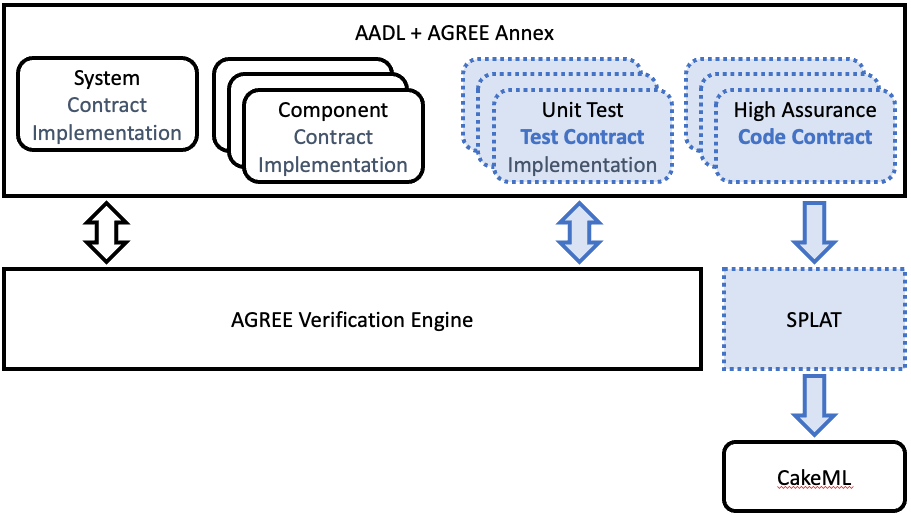
\includegraphics[width=0.8\textwidth]{flowchart.png} \\
    \end{tabular}
  \end{center}
\caption{A simplified illustration of the \brfcs\ toolkit with shaded portions being the contributions presented here.}
\label{fig:flowchart}
\end{figure*}

\begin{figure*}
	\begin{center}
	  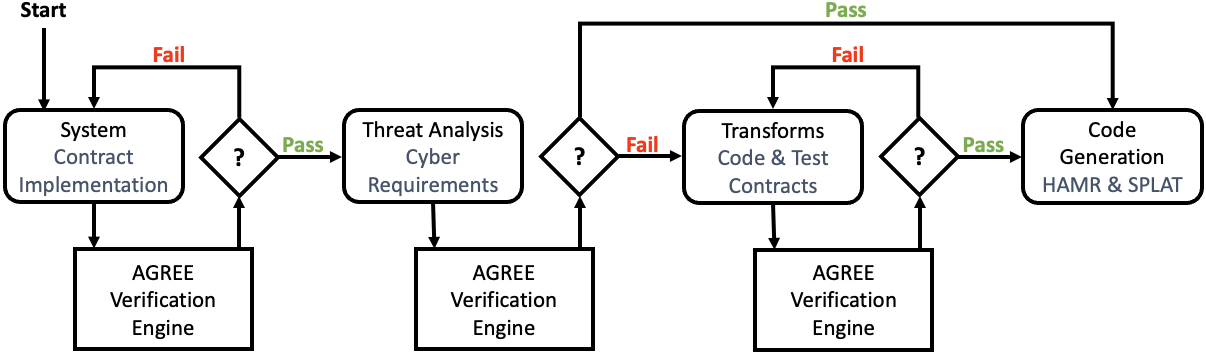
\includegraphics[width=\textwidth]{./figs/workflow.png}
  	\end{center}
	\caption{The general workflow for \brfcs.}
	\label{fig:workflow}
\end{figure*}

The \brfcs\ OSATE environment provides designers with workflow and tool support for developing products with
inherent cyber-resiliency.
%
\figref{fig:flowchart} is a simplified illustration of the toolkit that omits tooling outside of our contributions discussed here (see \cite{dcrypps2019,gearcase2020,resolute-destion,attestation-copland,awas,hamr,sel4-sosp09, sel4-tocs14, sel4-cacm18} for other aspects of \brfcs).
%
The shaded boxes represent our contribution: test contracts, code contracts, and SPLAT synthesis.
The unshaded boxes are the existing elements that provide the foundation for our contributions.

The intended \brfcs\ workflow is in \figref{fig:workflow}.
%
The workflow starts with a behavioral description of the system and its components on the left.
%
These descriptions are contracts that assume properties on inputs and guarantee properties on outputs when the input assumptions hold.
Once \agr\ verifies the system contract composition, the workflow moves right to the threat analysis, and the contracts of the system and components are modified to reflect that analysis.
%
If \agr\ verifies the system contract composition with the changes from the threat analysis, then the workflow moves to the far right for code generation.
%
Otherwise it moves immediate right to transforms.
Here the designer inserts high-assurance components such as filters and monitors, with their accompanying code contracts, until \agr\ verifies the new system composition to be cyber-resilient to the indicated threats.
%
Once \agr\ verifies the new system composition, the workflow moves to code generation, where \splt\ synthesizes implementations for the inserted high-assurance components from their corresponding code contracts.

We use this section to explain both figures in more detail through an example.
%
The example is a UAV system for remote monitoring, and it is loosely based on
the case study in \secref{sec:case-study}.
%
The source for the example is at \cite{repo}.
%
The intent of the UAV system is to receive a mission from the ground station, plan a path to fly that mission from its current location, and then fly the planned path updating the ground station along the way.
%
The system must by cyber-resilient and actively protect itself from malicious actors to ensure it is sending accurate monitoring information back to the ground station and that it actually flies the intended mission.

%%
% SYSTEM AND COMPONENT CONTRACT IMPLEMENTATION
%%

\subsection{System and Component Contract Implementation}

\begin{figure*}[h]
  \begin{center}
    \begin{tabular}{c}
      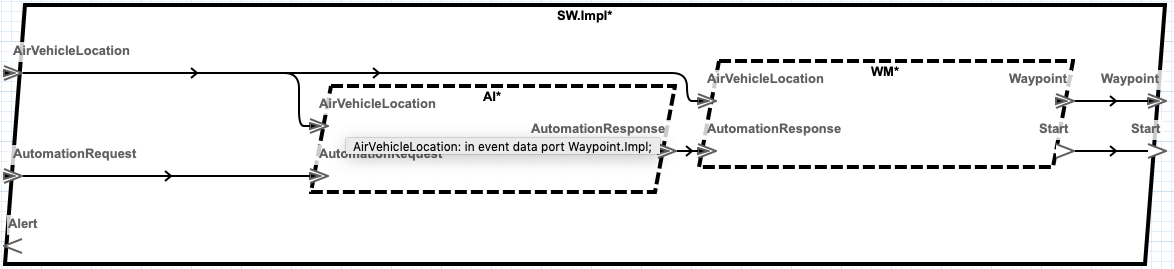
\includegraphics[width=\textwidth]{example.png}
    \end{tabular}
  \end{center}
\caption{Initial design for an automated UAV route planning system.}
\label{fig:example}
\end{figure*}

\begin{figure}
  \begin{center}
    \begin{tabular}{c}
      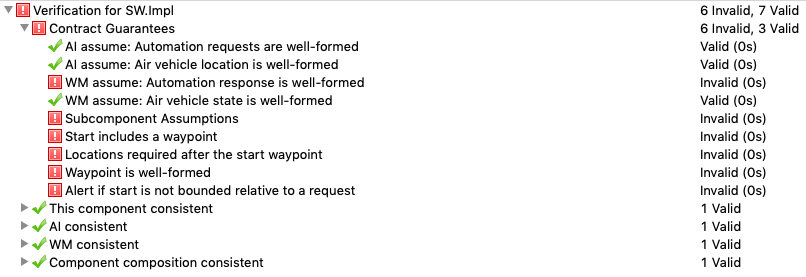
\includegraphics[width=1\columnwidth]{example-certificate.png} \\
    \end{tabular}
  \end{center}
\caption{\agr\ failure certificate for initial design.}
\label{fig:example-certificate}
\end{figure}

We focus on the software system for the UAV in this example.
%
The AADL architecture model for that system consists of two components as shown in \figref{fig:example}.
%
The first is the component for the automatic path planning for a mission (AI).
%
And the second is the component to meter the flight path waypoints to the actual UAV flight controller (WM).


From time to time, SW receives a message on the \texttt{AutomationRequest} input, forwarding it to the AI.
%
The function of AI is to compute the flight path (a list of waypoints) for the UAV, outputting the resulting \emph{mission command} on \texttt{AutomationResponse}.
%
The WM receives the mission command from AI and starts the UAV flying the mission by putting an \emph{event} on the \texttt{Start} output port, continuing to issue waypoints to the UAV flight controller on the \texttt{Waypoint} port as the UAV location updates with messages on \texttt{AirVehicleLocation}.
%
The AI component is third-party software and WM is a legacy component.

The expected behavior of the SW system, and the components implementing the system, are modeled with \agr\ contract specifications as shown by the unshaded boxes in the top-left of \figref{fig:workflow}.
%
These contracts assume and guarantee the absence of any malicious, or unspecified, component behavior.
%
More precisely, the contract for SW assumes that its inputs are \emph{well-formed} and that there is never more than one automation request pending at a time.
%
Well-formed generally refers to a syntactic restriction on data at a port. For example, a waypoint is well-formed if it falls within bounds for latitude, longitude, and altitude.
%
The guarantees for SW ensure that
\begin{compactitem}
\item a start coincides with a new waypoint being output;
\item a start is within one cycle of an automation request and if not, then it persistently alerts;
\item new waypoints coincide with location updates; and
\item all outputs are well-formed.
\end{compactitem}

The contracts for the sub-components assume their inputs are well-formed, and they guarantee their outputs are well-formed.
%
The AI contract guarantees it only responds to automation requests and always in the same cycle.
%
The legacy WM contract guarantees that
\begin{compactitem}
  \item it generates a start from a response from the AI and always in the same cycle;
  \item the start coincides with a waypoint; and
  \item any further waypoints coincide with location updates.
\end{compactitem}

This behavioral contract definition of the UAV software system is the starting point on the left-side of \figref{fig:workflow}.
%
The \agr\ verification engine tries to prove if the component composition of the software system is correct.
%
It is an iterative process where the designer updates contracts in the composition until \agr\ proves out the composition.
%
For our example, the initial specifications described above pass verification, meaning that the contract composition of the components with the system satisfies all component input assumptions and system output guarantees.
%
The \agr\ verification conditions, syntax and semantics, and the baseline contracts for the example are discussed in detail in \secref{sec:agree}.
%
\figref{fig:sw} in that section is the \agr\ contract for SW.

%%
% ADDING CYBER REQUIREMENTS
%%

\subsection{Adding Cyber Requirements}

Having passed \agr\ verification, the workflow in \figref{fig:workflow} proceeds to the thread analysis as the UAV must actively protect itself from malicious actors.
%
Threat analysis identifies the potential of a supply chain attack through the AI route planner since its third-party.
%
To mitigate the identified supply chain attack, the designer adds a requirement that the system must guard against malicious AI behavior.
%
This requirement is reflected in the component contracts by removing all output guarantees from the AI contract since that component is considered untrusted.
%
Without output guarantees, the AI component is able to output arbitrary events in the \agr\ verification analysis.

The output from that analysis is shown in \figref{fig:example-certificate}.
%
The red exclamation points designate component assumptions or system output guarantees that do not hold, and each failure comes with a corresponding counter-example.
%
The first violation is that the mission command on \texttt{AutomationResponse} from the AI to the WM is no longer guaranteed to be well-formed: the red exclamation point on \emph{WM assume: Automation responses are well-formed}.
%
The consequence of that failing input assumption is that the WM outputs are no longer guaranteed.
%
For a contract, when an input assumption does not hold, then the output may be arbitrary.
%
The rest of the failures in \figref{fig:example-certificate} are the result of the WM outputs now being arbitrary.

\begin{figure*}
  \begin{center}
    \begin{tabular}{c}
      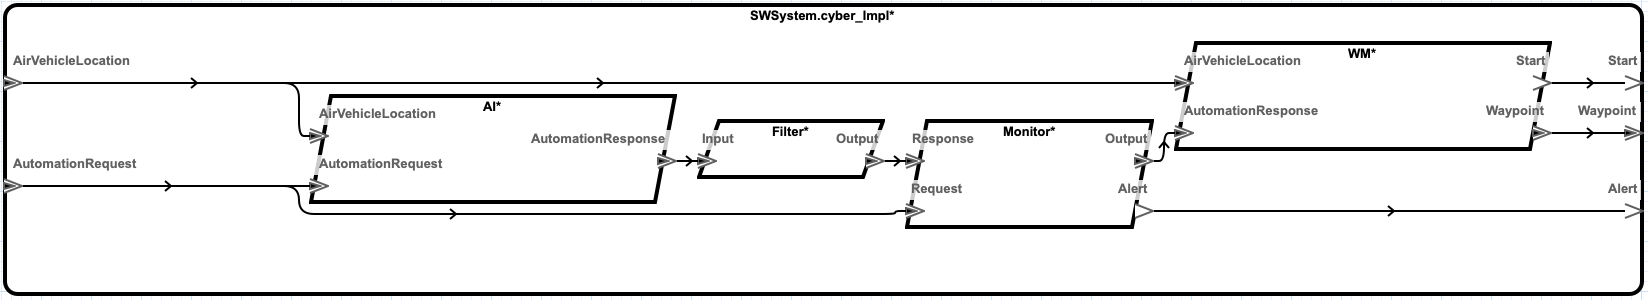
\includegraphics[width=2\columnwidth]{hardened.png}
    \end{tabular}
  \end{center}
  \caption{Cyber-hardened design for an automated UAV route planning system}
  \label{fig:hardened}
\end{figure*}

\begin{figure}
  \begin{center}
    \begin{tabular}{c}
      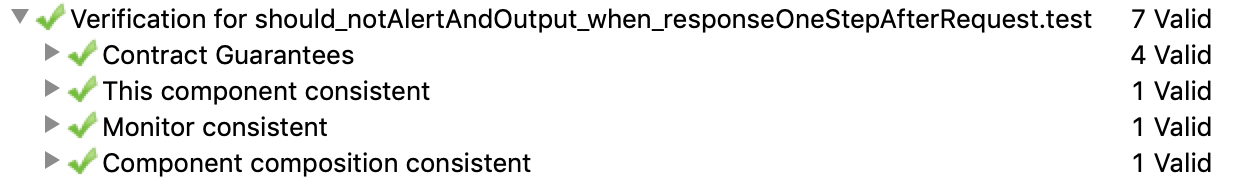
\includegraphics[width=\columnwidth]{agree-test-output.png} \\
      (a) \\ \\
      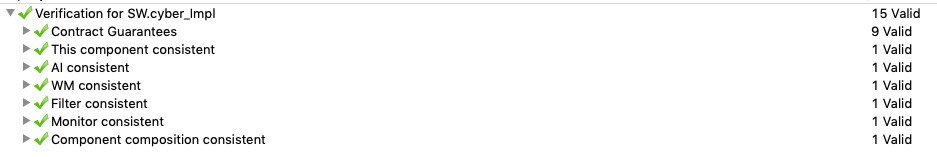
\includegraphics[width=\columnwidth]{hardened-certificate.png} \\
      (b)
    \end{tabular}
  \end{center}
  \caption{\agr\ verification certificates. (a) Test contract verification results. (b) Cyber-hardened design verification results.}
  \label{fig:hardened-certificate}
\end{figure}

%%
% ADDING HIGH ASSURANCE COMPONENTS
%%

\subsection{Adding High-assurance Components}

As \agr\ proves the system does not meet its cyber-requirements, the workflow moves to the right in \figref{fig:workflow} to the transforms box.
%
Here is where the shaded regions in \figref{fig:flowchart} come into play.
%
The system designer now uses \brfcs\ to cyber-harden SW by inserting high-assurance components in the form of a filter and a monitor, as shown in \figref{fig:hardened}.
%
These are intended to mitigate and report any observed malicious behavior by AI.

A filter enforces an invariant over each datum in the data stream by not forwarding input to its output if the invariant does not hold.
%
\brfcs\ generates an initial code contract for the filter which the designer completes by writing the invariant.
%
That invariant is usually based on the existing assumptions made by downstream components that consume the filter output.
%
In this example, it is the well-formed property for the automation request.

A monitor captures a relation on data over time and is thus able to reason about the temporal, and other invariant, properties of that data.
%
It raises an alert if the specified properties are ever violated.
%
As with the filter, \brfcs\ generates an initial code contract that is completed by the designer.
%
In this example, that contract states that an automation response can only be generated in conjunction with an automation request;
%
and further, that response must come with the request or in the next step after the request.
%
Code contracts are discussed in detail in \secref{sec:code-contracts}.
%
\figref{fig:filter} and \figref{fig:monitor} are the code contracts from that section for the high-assurance filter and monitor inserted into the original system as shown in \figref{fig:hardened}.

Code contracts for high assurance components can be arbitrarily complex since they can have persistent state that evolves over time.
%
Test contracts allow the designer to validate code contract behavior with unit testing.
For example, one of the test contracts for the monitor is that when it sees an automation response one step after a request, then it should not alert, and it should pass the response downstream.
%
Test contracts are discussed in detail in \secref{sec:testing}.
%
\figref{fig:test} in that section is an example test contract for the added monitor in our example.

As shown in \figref{fig:workflow}, making the system cyber-resilient is an iterative process of adding high-assurance components, writing their code contracts, testing those contracts with test contracts, and then seeing if they are sufficient to prove out the system.
%
The \agr\ analysis of the cyber-hardened implementation at the end of that iterative process is shown in \figref{fig:hardened-certificate}.
%
\figref{fig:hardened-certificate}(a) is the test contract results and \figref{fig:hardened-certificate}(b) is the hardened system composition.
%
Here \agr\ has generated high-level evidence justifying the claim that the high-assurance components meet their intended purposes.

%%
% SYNTHESIZING CODE FROM CODE CONTRACTS
%
\subsection{Synthesizing code from code contracts}

As \agr\ proves the system now meets its cyber-requirements, the workflow moves to the right in \figref{fig:workflow} to the code generation box.
%
High-assurance components are automatically synthesized by \splt\ from the code contracts to equivalent programs in the \ckml\ language.
%
In other words, for any set of input streams that meet the component's contract assumptions, the output streams produced from the synthesized \ckml\ code exactly match those defined by the contract guarantees.

The synthesis algorithm is a sequence of semantics preserving transforms that refine the code contract to a step function over the inputs and current component state. The function computes the next state and outputs for the component at each scheduling step.
%
As such, the \agr\ verification results regarding the code contract apply equally to the synthesized \ckml, and thus, the results equally apply to the resulting binaries from the \ckml\ compiler.
%
Synthesis from code contracts is discussed in detail in \secref{sec:synthesis}.
%
\figref{fig:filter-cakeml} and \figref{fig:monitor-cakeml} are the implementations from that section for the high-assurance filter and monitor from our example here.


Extending the \agr\ verification results to the system composition requires additional guarantees not discussed here.
%
For example, among other things, contracts for non-synthesized components must be certified to accurately model their deployed counterparts, the generated scheduler must be certified to follow the dependent data-flow in the design, scheduling windows must be certified to cover worst-case execution times, \etc.
%
Such additional guarantees are discussed in other works \cite{gearcase2020, dcrypps2019, 10.1007/978-3-030-89159-6_18, 10.1007/978-3-030-89159-6_17, sel4-2009, nfm:agree, 9734792}.

Our discussion so far regarding the role of \agr\ in \brfcs\ in \figref{fig:flowchart}, and its expected workflow in \figref{fig:workflow}, has been high-level and abstract.
%
Indeed, we have only given a birdseye view of how \agr\ supports the verification of the system, code contracts, and test contracts, as well as how it provides the proof results that underpin our claim that the synthesized high-assurance components guarantee the \agr\ verification results.
%
In the following sections we delve into the details of \agr, including its notation, semantics, and usage, to set the stage for our primary contributions in \secref{sec:code-contracts}, \secref{sec:testing}, and \secref{sec:synthesis}.
%
For reference to where we discuss the actual contracts for the example system, \secref{sec:sw-contract} is the exposition of the \agr\ contract for the SW component, \secref{sec:ha-contracts} is the exposition of the code contracts for the high-assurance filter and monitor shown in \figref{fig:hardened}, and \secref{sec:testing} includes an exposition of a test contract for the monitor.

%%
% AGREE
%%

\section{\agr}
\label{sec:agree}

\newcommand{\globally}{\konst{Always}}
\newcommand{\historically}{\konst{Hist}}
\newcommand{\assumes}{\ensuremath{A}}
\newcommand{\guarantees}{\ensuremath{P}}
\newcommand{\inputs}{\ensuremath{I}}
\newcommand{\outputs}{\ensuremath{O}}
\newcommand{\components}{\ensuremath{C}}
\newcommand{\component}{\ensuremath{c}}

The \agr\ specification language, and semantics, are inspired by the Lustre language \cite{10.1145/41625.41641}.
%
Lustre semantics are synchronous data-flow where the inputs and outputs of components are streams.
%
Informally, streams assign values to expressions at each point in time.
%
\agr\ contracts express relationships between input and output streams by assuming a set of allowed input streams and then guaranteeing a corresponding set of allowed output streams.

%%
% COMPONENTS
%%

\subsection{Components}

A system implementation is described by its ports, its subcomponents, and the connections between ports on different subcomponents.
%
Ports in \agr\ are inherited from AADL.
%
There are three kinds of port: \emph{event} ports, \emph{data} ports, and \emph{event data} ports.
%
An event port carries no data and only signals occurrence (or not) of the event.
%
A data port is a sampled port: the data can be read at anytime.
%
An event data port indicates when data is present with an event.

Data flows through the subcomponents of a system in dependency order, with inputs being propagated to outputs through all contracts until they stabilize \ie, cannot propagate further.
%
Therefore, subcomponent contracts, and thus the top-level model, must be acyclic.
%
Cyclic systems are made acyclic by breaking cycles with delays.
%
Once the data propagation has stabilized, the model proceeds to the next input data in the input streams.
%
It is worth noting that the semantics do not model computation or communication delay: the output of one contract is seen at the input of any downstream contract in the same step of the input data stream.

%%
% CONTRACTS AND VERIFICATION CONDITIONS
%%

\subsection{Contracts and verification conditions}

From the system and component contracts, \agr\ generates a set of verification conditions to show that a system's component implementation is correct~\cite{agree2013}.
%
The \agr\ model checker is then invoked to prove or disprove the verification conditions.
%
The contracts and verification conditions are expressed in \emph{past-time linear temporal logic} (PLTL) \cite{10.1093/jigpal/8.1.55}.

PLTL is a logic enhanced with temporal operators able to reason about the truth values of formulas through time.
%
It combines past-time operators that reason over the history of computation up to a point (PTLTL) and future-time operators that reason over the computation that follows that point (LTL).
%
Its semantics are defined relative to a point in time $i$, a finite trace of system states $\pi = s_0, s_1, \ldots, s_i$, and some logic formula $f$.

The two PLTL operators necessary for the \agr\ generated verification conditions are $\globally$ that looks forward in time along the trace and $\historically$ (historically) that looks backward in time along the trace.
%
These are defined as
%
\begin{eqnarray*}
 (\pi, i) \models \globally(f) & \iff & \forall j \ge i, (\pi, j) \models f \\
(\pi, i) \models \historically(f) & \iff & \forall 0 \le j \le i, (\pi, j) \models f
\end{eqnarray*}
%
The $\models$-operator is read as \emph{satisfies}.
%
A trace at a moment in time satisfies $\globally(f)$ if and only if it satisfies $f$ in the current and all future states of $\pi$.
%
$\globally(f)$ is invariant from the current moment into the future and $\historically$ is invariant from the beginning of the trace to the current moment.

A \emph{system} is a tuple $(\inputs, \outputs, \assumes, \guarantees,C)$, where $\inputs$ is the input set, $\outputs$ is the output set, $\assumes$ is the set of assumptions, $\guarantees$ is the set of guarantees, and $C$ are subcomponents.
%
Assumptions and guarantees only use the past-time operators from PLTL.
%
A subcomponent $\component$ is, hierarchically, also a system, and may be designated by its own tuple $(\inputs_\component, \outputs_\component, \assumes_\component, \guarantees_\component, C_c)$.
%
From the components and their connections, $\mathbb{I}_\component$ is defined to be the set of components providing input to some component $\component$ in the system, and $\mathbb{O}$ is defined to be the set of components that provide the output for the system.

A system is \emph{correct} if and only if for all components $c \in C$ the following two verification conditions hold:
%
\begin{equation}\label{eq:assumes}
            \globally(\historically(\assumes \wedge
            \bigwedge_{\component^\prime \in \mathbb{I}_\component} P_{\component^\prime})
            \implies \assumes_\component)
\end{equation}
%
\begin{equation}\label{eq:guarantees}
            \globally(\historically(\assumes \wedge
            \bigwedge_{\component^\prime \in \mathbb{O}} \guarantees_{\component^\prime})
            \implies \guarantees)
\end{equation}
%
The conditions from \eqref{eq:assumes} verify the input assumptions on each component under the system assumptions and upstream component guarantees.
%
They check if the component guarantees and system assumptions are strong enough to imply input assumptions on all immediate downstream components.
%
The condition in \eqref{eq:guarantees} checks the output guarantees of the system under the system assumptions and component guarantees that provide the output.
%
It checks if the guarantees on components providing primary outputs are strong enough to imply the system guarantees.

If all the verification conditions hold (\agr\ uses $k$-inductive model checking to automatically prove or disprove each generated verification condition), then the system is said to be \emph{correct}, meaning that the system composition meets input assumptions at each input as well as the guarantees on the system output.
%
A consequence of this result is that $\globally(\historically(\assumes) \implies \guarantees)$ holds for the system contract.
%
Therefore the Liskov substitution principle applies and the implementation is a safe substitution for the system contract \cite{10.1145/62139.62141}.

The expanded property lists in \figref{fig:example-certificate} and \figref{fig:hardened-certificate} are the results from verifying or disproving the above verification conditions.
%
The additional unexpanded results at the bottom of the figures prove \emph{self-consistency} in the contracts.
%
A contract is self-consistent if it does not guarantee two different values in the same moment of time, \ie, the contract is not self-contradicting.
%
\agr\ generates additional verification conditions that prove each component contract, and the composition of contracts, self-consistent.

%%
% SYNTAX
%%

\subsection{Syntax}
\label{sec:agree-semantics}

The syntax of \agr\ is essentially that of quantifier-free first order predicate logic supplemented with a few temporal operators.
%
The terms (\emph{e}) are arithmetic expressions built from variables ($v$) and numeric and boolean literals ($c$), while formulas (\emph{b}) are built using logical connectives from atomic formulas (\emph{a}) based on the familiar comparison operators.
%
\[
\begin{array}{rcl}
e & ::= & v \mid c \mid e \;\set{+,*,/}\; e \\
a & ::= & e\; \set{=,<}\; e \\
b & ::= & v \mid c \mid a \mid \neg b
            \mid b \; \set{\land,\lor,\imp,\iff}\; b
\end{array}
\]
%
\agr\ includes a conditional, $\itelse{b}{(-)}{(-)}$, for both terms and formulas. To support port handling, \agr\ defines a predicate $\konst{event}(p)$, which tests if an event (or event-data) port $p$ is signaled.
%
Lastly, \agr\ supports temporal operators \emph{previously} $\konst{pre}(-)$, \emph{followed-by} $(-) \to (-)$, and historically $\konst{Hist}(-)$.

%%
% SEMANTICS
%%

\subsection{Semantics}

The semantics of terms and formulas is defined over \emph{streams of values}.
%
Values encompass at least booleans and numbers but can be readily extended to include records and arrays.
%
A value stream is a total function from time (natural numbers including 0) to values:
%
\[
 \konst{stream} = \mathbb{N}_0 \to \konst{value}
\]
%
Given an \emph{environment} $E : \konst{name} \mapsto \konst{stream}$ binding variable names to value streams, the semantics $\sem{-}^E_t$ of terms and formulas defines the meaning of compound syntax in terms of the meaning of subexpressions.
%
The value of a variable $v$ at time $t$ is found by looking up the stream bound to $v$ in $E$ (call it $s$) and returning $s_t$. Some clauses of the semantics follow, omitting the temporal operators:
%
\[
\begin{array}{rcl}
\sem{v}^E_t & = & E(v)(t) \\
\sem{c}^E_t & = & c \\
\sem{e_1 + e_2}^E_t & = & \sem{e_1}^E_t + \sem{e_2}^E_t \\
   & \cdots & \\
\sem{b_1 \land b_2}^E_t & = & \sem{b_1}^E_t \land \sem{b_2}^E_t \\
   & \cdots & \\
\end{array}
\]

The temporal operators deal with time in more significant ways.
%
The value of $\konst{pre}(e)$ at time $t$ is the value of $e$ at time $t-1$ (at time zero, \konst{pre} is undefined).
%
A followed-by, $e_1 \to e_2$, evaluates to $e_1$ at time zero; otherwise it is $e_2$.
%
Followed-by is typically used to give a value to a stream in the first step so that subsequent steps are able to use $\konst{pre}(e)$.
%
\[
\begin{array}{rcl}
\sem{\konst{pre}(e)}^E_t & = & \sem{e}^E_{t-1}, \mathrm{when}\ t > 0 \\
\sem{e_1 \to e_2}^E_t & = & \itelse{t=0}{\sem{e_1}^E_0}{\sem{e_2}^E_t} \\
\sem{\konst{Hist}(b)}^E_t & = & \forall n \leq t.\; \sem{b}^E_n
\end{array}
\]

Although basic, these definitions can be used to define higher-level past-time operators from PLTL such as \konst{Once} and \konst{Since}.
%
These can be expressed in a recursive style as follows:
%
\[
\begin{array}{rcl}
\konst{Once}(b) & = & b \to b \vee \konst{pre}(\konst{Once}(b)) \\
\konst{Since}(a, b) & = & b \to b \lor (a \land \konst{pre}(\konst{Since}(a, b))
\end{array}
\]
%
\noindent $\konst{Once}(b)$ is true if $b$ has ever been true before, or in, the current moment.
%
$\konst{Since}(a, b)$ is true if $a$ has been true in all moments up to the present one since $b$ most recently became true.
%
All other past-time operators of PLTL can be defined similarly \cite{monitor}.

\agr\ uses ASCII notation for the mathematical syntax we have defined.
%
The following table spells out the mapping.
%
\[
\begin{tabular}{l|l|l}
 Operation & Math. notation & \agr \\ \hline
 followed-by &  $e \to e$          & \verb+e -> e+  \\
 logical implication &  $e \imp e$ & \verb+e => e+ \\
 if-and-only-if &  $e \iff e$      & \verb+e <=> e+ \\
 logical and &  $e \land e$      & \verb+e and e+ \\
 logical or &  $e \lor e$      & \verb+e or e+ \\
 logical not & $\neg b$      & \verb+not b+ \\
 variable definition & $v = e$     & \verb+eq v e+ \\
 Previously  & $\konst{pre}(b)$ & \verb+pre(b)+ \\
 Historically  & $\konst{Hist}(b)$ & \verb+Historically(b)+ \\
\end{tabular}
\]

%%
% FORMAL CONTRACT FOR THE EXAMPLE SYSTEM
%%

\subsection{Formal contract for the example system}
\label{sec:sw-contract}

\newsavebox{\sw}
\begin{lrbox}{\sw}
\begin{lstlisting}[style=agree,numbers=left]
eq req : bool = event(AutomationRequest);*\label{line:sw-event-def-start}*
eq avl : bool = event(AirVehicleLocation);
eq wp  : bool = event(Waypoint);
eq strt: bool = event(Start);
eq alrt: bool = event(Alert);*\label{line:sw-event-def-end}*

assume "Automation requests are well-formed" : *\label{line:sw-assume-1}*
  req => WELL_FORMED_AUTOMATION_REQUEST(AutomationRequest);
assume "Air vehicle locations are well-formed" : *\label{line:sw-assume-2}*
  avl => WELL_FORMED_WAYPOINT(AirVehicleLocation);
assume "One automation request in flight at a time" : *\label{line:sw-assume-3}*
  true ->
  (req => pre(Historically(not req) or Since(not req, strt)));

guarantee "Waypoints coincide with air vehicle locations": *\label{line:sw-guarantee-1}*
  wp => avl;
guarantee "Starts include a new waypoint" : *\label{line:sw-guarantee-2}*
  strt => wp;
guarantee "Waypoints are well-formed" :  *\label{line:sw-guarantee-3}*
  wp => WELL_FORMED_WAYPOINT(Waypoint);
guarantee "Starts within one cycle of requests if not alerting" : *\label{line:sw-guarantee-4}*
  (strt => ((not alrt) and req)) ->
  (strt => ((not alrt) and (req or pre(req))));
guarantee "Alert if not started within one cycle of requests" : *\label{line:sw-guarantee-5}*
  true -> ((pre(req and not strt) and not strt) => alrt);
guarantee "Once alerted always alerted" : *\label{line:sw-guarantee-6}*
  Once(alrt) => alrt;
\end{lstlisting}
\end{lrbox}

\begin{figure}
  \begin{center}
    \scalebox{0.62}{\usebox{\sw}}
  \end{center}
  \caption{The SW component contract.}
  \label{fig:sw}
\end{figure}

The AGREE specification for the SW component in \secref{sec:example} is given in \figref{fig:sw}.
%
\linesref{line:sw-event-def-start}{line:sw-event-def-end} define local variables that are true when data is present on the corresponding event ports for the component.  These variables are
purely for notational convenience.
%
The contract has three assumptions:
%
\begin{itemize}
\item
\lineref{line:sw-assume-1} and \lineref{line:sw-assume-2}.
%
When input is present it is well-formed.
%
The well-formed predicates are defined elsewhere using AGREE functions.

\item
\lineref{line:sw-assume-3}.
%
If there is an incoming request, it is either the very first one, \texttt{\textbf{Historically}(\textbf{not} req)}, or it arrives after the component has output a start event in response to a previous request, \texttt{\textbf{Since}(\textbf{not} req, strt)}---to be read as \emph{not
request since start}.
\end{itemize}

\noindent The contract has six guarantees:
%
\begin{itemize}
\item
\lineref{line:sw-guarantee-1}, \lineref{line:sw-guarantee-2}, and \lineref{line:sw-guarantee-3}.
%
A waypoint coincides with a update on the UAV location, a start coincides with a new waypoint, and waypoints are well-formed.

\item
\lineref{line:sw-guarantee-4}.
%
A start happens with a request or one step after a request.
%
At time zero the start must coincide with the request;
%
after that, the start must coincide with the request or else is a response to a request one step earlier.
%
The guarantee works with the assumption on \lineref{line:sw-assume-3} and thus does not have to check for two requests in a row without a start, since the assumption precludes that input behavior.
%
The guarantee also does not force the start to always happen, it only says that if it does happen, it is under the defined conditions.

\item
\lineref{line:sw-guarantee-5}.
%
The alert is signaled if the start does not arrive within the one-step bound.
%
Together with \lineref{line:sw-guarantee-4} this allows for non-alerting and alerting behavior.

\item
%
\lineref{line:sw-guarantee-6}.
%
If an alert has ever happened, it continues to happen.
\end{itemize}
%
These six guarantees define the behavior of the SW component under the three assumptions and correspond to the informal descriptions given in \secref{sec:example}.

\section{Code contracts for high assurance components}
\label{sec:code-contracts}

Generally, AGREE contracts do not describe the computation that a component performs.
%
This is entirely by design: AGREE is intended to be declarative and reasoning about component behavior takes place solely at the specification level.
%
It defines what a component computes and not how it computes it.
%
However, the syntax of AGREE provides enough expressiveness to support the notion of a \emph{code contract}: a contract from which an implementation can be extracted.
%
First we must discuss a class of guarantees, \emph{output guarantees}, which determine the values on all output ports of a component.

\begin{definition}[Output guarantee]
An \emph{output guarantee} is a stylized guarantee that fully specifies the data written to an output port.
%
There are three possibilities according to whether the output port $p$ is a \konst{data} port, an \konst{event} port, or an \konst{event data} port:
%
\[
\begin{array}{ll}
\konst{data}: &  p = \mathit{e} \\
\konst{event}: &  \konst{event} (p) = \mathit{b} \\
\konst{event data}: & \itelse{b}{\konst{event} (p) \land p = e}{\neg \konst{event}(p)} \\
\end{array}
\]
%
\end{definition}

Informally, a code contract treats its \konst{eq} ``statements'' as defining a list of assignments to state variables, and its output guarantees as directives for producing output.

\begin{definition}[Code contract]
A leaf component of the form $(I,O,A,P,\emptyset)$ is a \emph{code contract} if $\mathit{Eqs} \cup G \subseteq P$, where \[\mathit{Eqs} = \set{v_1 = e_1, \cdots , v_n = e_n} \] is a non-empty set of \konst{eq} statements and $G$ is the set of output guarantees, one for each element of $O$.
%
In the interpretation as code, the order of elements of $\mathit{Eqs}$ is important, and is simply taken to be the occurrence order of the \konst{eq} statements in the syntax.
%
Thus we will work with the \emph{list} of equations $\mathit{Eqs} = [v_1 = e_1; \cdots ; v_n = e_n]$.
\end{definition}

The semantics of \secref{sec:agree-semantics} supports a formal connection between the original contract, and verification results of the AGREE model checker being run on it, and code generated from specifications of leaf level cyber-components.
%
It also provides the root meaning at the base of a chain of translation steps moving from an AGREE contract to a CakeML executable.

The first step in the chain maps the contract to a code-focused representation.
Assume given a code contract $(I,O,A,\mathit{Eqs} \cup G \cup P,\emptyset)$, environment $E$, and time $t$.
%
The \emph{evaluation} of $\mathit{Eqs}$ followed by the evaluation of $G$ results in a new environment $E'$ where the stream values for state variables and outputs have been computed for time $t$.
%
The step from $E$ to $E'$ is one full cycle in the repeated evaluation of the component.

\begin{definition}[Evaluation]
We overload existing notation and write the evaluation of $\mathit{Eqs}$ and then $G$ in environment $E$ at time $t$ as $\sem{\mathit{Eqs}\cdot G}^E_t$.
%
The evaluation of $v = e \in {\Eqs}$ is an environment transformation
%
\[
 \sem{v = e}^E_t = E[v(t) \mapsto\sem{e}^E_t] \ .
\]
%
modifying $E$ so that stream $v$ has value $\sem{e}^E_t$ at time $t$.
%
The list {\Eqs} is evaluated by folding the transformation left-to-right through it.
%
The transformation is similarly applied to the list of output guarantees $G$, computing the values on output ports.
%
The details are omitted, being a bit messy because of the different kinds of output ports available.
\end{definition}

\begin{definition}[Code contract correctness]
Assume code contract $(I,O,A,\mathit{Eqs} \cup G \cup P,\emptyset)$.
%
The contract is \emph{correct}, if for all $E$ and $t$, whenever the assumptions (historically) hold in $E$ and evaluation steps from $E$ to $E'$, then the guarantees hold in $E'$:
%
\[
\sem{\konst{Hist}(A)}^E_t \land E' = \sem{\mathit{Eqs} \cdot G}^E_t \imp \sem{P}^{E'}_t
\]
%
\end{definition}

How does this notion of correctness integrate with the verification conditions generated by AGREE?
%
In \emph{contract correctness}, the model checker is proving the following property
%
\[
\konst{Hist}(A) \imp P
\]
%
and in \emph{code contract correctness} we essentially prove a Hoare triple of the form
%
\[
\set{\konst{Hist}(A)}\; (\mathit{Eqs} \cdot G) \; \set{P}
\]
%
This accords with intuition, namely that AGREE is a kind of \emph{program-free program logic};
%
by pulling out a program $(\mathit{Eqs}\cdot G)$ from a code contract we find ourselves in the domain of imperative program verification.
%
For example, at this point one could apply a verification condition generator to help break down the proof obligation.
%
In order to use the code contract result in system contract verification conditions, one has to show that the code contract result implies the system verification condition.

%%
% IMPERATIVE CODE CONTRACTS
%%

\subsubsection*{Imperative code contracts}

Stream-based evaluation allows values arbitrarily \emph{deep in the past} to be accessed by use of $\konst{pre}(-)$.
%
However, the programming languages targeted by SPLAT do not directly support streams.
%
We are developing a translation to eliminate such deep temporal accesses by the introduction of intermediate variables.
%
The essential property the translation needs to satisfy is a syntactic restriction, call it \emph{Pascal-like}, that supports easy translation to standard imperative languages.
%
The guiding intuition is that a Pascal-like {\Eqs} accesses at most one step in the past;
%
also, accesses to a past value of a variable are only possible until the variable is updated.
%
In informal terms, this means that ${\Eqs}\cdot G$ in a code contract has the following properties:
%
\begin{itemize}
\item Followed-by only occurs at the top level of a variable definition, \eg, $v = e_1 \to e2$;
\item $\konst{pre}(e)$ is allowed only when $e$ is a variable; and
\item $\konst{pre}(v)$ is allowed only before the defining equation $v = e$ (and may occur in $e$).
\end{itemize}
%
For example, the Fibonacci sequence $1,1,2,3,5,8,13,\ldots$ can be defined, albeit in a manner that is not Pascal-like, by
%
{\small
\begin{lstlisting}[style=agree]
  Fib = 1 -> pre(1 -> Fib + pre Fib)
\end{lstlisting}
}
%
\noindent or by (again this is not Pascal-like)
%
{\small
\begin{lstlisting}[style=agree]
  N = 0 -> 1 + pre(N)
  Fib = if N <= 1 then 1 else pre(Fib) + pre(pre(Fib))
\end{lstlisting}
}
%
\noindent or by (this time Pascal-like):
%
{\small
\begin{lstlisting}[style=agree]
  N = 0 -> 1 + pre(N)
  F2 = 42 -> pre(F1)
  F1 = 42 -> pre(Fib)
  Fib = if N <= 1 then 1 else F1 + F2
\end{lstlisting}
}
%
Please note that the initial values of \verb+F1+ and \verb+F2+ are never accessed, so 42 could be replaced by any number in their defining equations.
%
A Pascal-like ${\Eqs} \cdot G$ is straightforward to implement in conventional programming languages, as we will see in \secref{sec:synthesis}.

\subsection{Code contracts for the hardened system}
\label{sec:ha-contracts}

\newsavebox{\flt}
\begin{lrbox}{\flt}
  \begin{lstlisting}[style=agree,numbers=left] -- start user
    -- start user definitions
    eq policy : bool =
      WELL_FORMED_AUTOMATION_RESPONSE(Input);
    -- end user definitions

    guarantee "Filter output is well-formed" :
      if event(Input) and policy then
        event(Output) and Output = Input
      else
        not event(Output);
  \end{lstlisting}
\end{lrbox}

\newsavebox{\mntr}
\begin{lrbox}{\mntr}
  \begin{lstlisting}[style=agree,numbers=left]
    const is_latched : bool = true;

    -- start user definitions
    assume "One automation request in flight at a time" : *\label{line:mon-assume}*
      true -> (req => pre(Historically(not req) or Since(not req, rsp)));

    const MAX_LATENCY : int = 1; *\label{line:mon-const}*

    eq rsp : bool = event(Response);
    eq req : bool = event(Request);

    eq preIsPending : bool = false -> pre(isPending);*\label{line:mon-pre-pending}*
    eq isPending : bool = Since(not rsp, req and not rsp);*\label{line:mon-pending}*
    eq latency : int = 0 -> (if req then 0 else pre(latency) + 1);*\label{line:mon-latency}*

    eq policy : bool = (rsp => req) -> *\label{line:mon-policy}*
                         (    (isPending => latency < MAX_LATENCY)
                          and (rsp => (req or preIsPending)));
    -- end user definitions

    eq alert : bool = (not policy) -> *\label{line:mon-alert}*
                        ((is_latched and pre(alert)) or not policy);

    guarantee "Alert port tracks alert variable" :
      event(Alert) = alert;
    guarantee "Output if not alerted" :
      if (not(alert) and rsp) then
          event(Output) and (Output = Response)
      else
          not (event(Output));
  \end{lstlisting}
\end{lrbox}

\begin{figure}
  \begin{center}
    \begin{tabular}{c}
      \scalebox{0.62}{\usebox{\flt}} \\
    \end{tabular}
  \end{center}
  \caption{Code contract for high-assurance filter.}
  \label{fig:filter}
\end{figure}

\begin{figure}
  \begin{center}
    \begin{tabular}{c}
    \scalebox{0.62}{\usebox{\mntr}} \\
    \end{tabular}
  \end{center}
  \caption{Code contract for high-assurance monitor.}
  \label{fig:monitor}
\end{figure}

Code contracts for the filter and monitor are shown in \figref{fig:filter} and \figref{fig:monitor}.
%
The filter is direct: it defines the policy according to the well-formed requirement for data.
%
We now discuss the monitor in some detail.

The monitor informally behaves as follows: if the \emph{policy} is obeyed in the current step, and the alert has not yet been raised, then the \texttt{Response} input is sent out on \texttt{Output}, and the \texttt{Alert} output stays low \lineref{line:mon-alert}.
%
Otherwise \texttt{Alert} goes high and stays high, and there is nothing sent henceforth on \texttt{Output}.

The \texttt{alert} variable (distinct from the \texttt{Alert} port) depends not just on the policy but also on the \texttt{is\_latched} constant, which has been set at configuration time.
%
Since \texttt{is\_latched} is \konst{true}, the alert is persistent, meaning that once the alert is raised, it is always raised;
%
otherwise, it is the complement of the policy value in the current step.

The monitor policy is defined by marking, with variable \texttt{isPending}, when a request is made but not yet satisfied, and by counting the number of steps (\texttt{latency}) between requests.
%
See \linesref{line:mon-pre-pending}{line:mon-latency}:
%
The \texttt{isPending} variable is true whenever there is a request that does not coincide with a response, \ie, \texttt{isPending} holds when \emph{there is no response since the most recent request without a corresponding response}.
%
The \texttt{latency} variable starts at zero, resets on every request, and otherwise increments by one.  Note that the \texttt{preIsPending} variable is a temporary needed to make the contract Pascal-like;
%
otherwise, the current and previous value of \texttt{isPending} would be simulataneously accessed in the definition of \texttt{policy}.

The policy (\lineref{line:mon-policy}) makes sure the latency is bounded whenever there is a pending request, and it ensures that a response is a result of a request.
%
The initial step differentiates from later steps in only needing to be sure a response is a result of a request, both happening in the initial step.

The latency bound for the monitor is defined by the constant \texttt{MAX\_LATENCY} (\lineref{line:mon-const}).
%
In this example the constant is set to one to be consistent with the system specification from the previous section.
%
At time zero the policy is trivial: a response requires an accompanying request.
%
After time zero, if a request is pending in the current time step, then the latency must still be under the bound, and if there is a response, then it closes a request now or a pending request from earlier in time.

The policy definition only works if there is never more than one outstanding request at a time;
%
otherwise, the latency counter resets incorrectly.
%
That requirement is encoded in the assumption (\lineref{line:mon-assume}) and is the same assumption used for the system input.
%
In fact, the policy can be written without the assumption, but the policy is much simpler to write with the assumption.

As shown in \figref{fig:hardened-certificate}, the cyber-hardened system passes AGREE verification.
%
That means that the high-assurance components protect the WM from the untrusted AI generating malformed data, spontaneous responses, or delayed responses.
%
Synthesis must generate faithful implementations of the code contracts for the AGREE verification result to apply to the deployed system.

%%
% TEST CONTRACTS
%%

\section{Test contracts}
\label{sec:testing}

Writing and proving properties about code contracts is difficult because it is a formal process, and because it reasons about constraints that define the entire input space, and the entire output space, of a high-assurance component at once.
%
Case studies have shown that designers, as well as formal method practitioners, make mistakes writing these contracts, especially if the computation or temporal reasoning in the contract is complex.

We have observed three common types of mistakes in code contracts (aside from self-consistency, which is already checked): vacuity, under-specification, and missed corner cases.
%
Vacuity is a common pitfall with implication when the left hand side is always false, making the implication true.
%
Under-specification is very challenging, as \agr\ is not able to prove anything (or it can prove everything in the case of existential properties), so nothing is actually known after verification except that the contract is under-specified.
%
Missed corner cases is a common problem to all disciplines.
%
It is an especially difficult challenge here because there is no direct way to exercise code contracts, \eg, there is no runtime \emph{per se}.

A tempting approach to exercising code contracts directly is to use \splt\ to create the target binary and then use that runtime with traditional testing.
%
Such an approach adds extra steps, including test harneses, that are not needed, as it is possible to bridge the formal model in \agr, with its proof system, to traditional validation using tests.
%
The intuition for that bridge comes from the compositional reasoning in AADL and \agr.
%
Effectively, a code contract for a high assurance component should be a valid implementation of a test scenario.
%
In other words, the test scenario, as expressed in a test contract, is the desired behavior of the system, and the code contract implements that behavior.

A test contract defines the test scenario for the code contract to implement.
%
It does this by assuming the test input and guarantying the test output akin to a unit test.
%
The code contract is used as the implementation, \eg, it is the test subject.
%
The \agr\ analysis then proves if the code contract, given the test inputs, is strong enough to prove the test contract outputs.
%
Here the test contract assumptions strengthen the code contract assumptions to a single input, and the test contract guarantees weaken, or leave unchanged, the code contract output for that test input, depending on the goal of the test.
%
In other words, according to Liskov substitution, \agr\ proves if the code contract is a safe substitution for the test contract.

\newsavebox{\tst}
\begin{lrbox}{\tst}
  \begin{lstlisting}[style=agree,numbers=left]
    process should_notAlertAndOutput_when_responseOneStepAfterRequest
      ... -- Omitted AADL features
      annex agree {**
        eq index : int = prev(index + 1, 0); *\label{line:tst-index}*

        assume "One Response one step after Request" : *\label{line:tst-assume-1}*
                ((index = 0) => not event(Response))
            and ((index = 1) => event(Response))
            and ((index >= 2) => not event(Response));
        assume "One Request" : *\label{line:tst-assume-2}*
            (event(Request) = true) ->
            (event(Request) = false);

        guarantee "Not Alert" : *\label{line:tst-guarantee-1}*
            not event(Alert);
        guarantee *\label{line:tst-guarantee-2}*
          "Output one step after Request at same time as Response" :
                ((index = 0) => not event(Output))
            and ((index = 1) => (event(Output) and Output = Response))
            and ((index >= 2) => not event(Output));
      **};
    end should_notAlertAndOutput_when_responseOneStepAfterRequest;

    process Implementation *\label{line:tst-imp-start}*
      should_notAlertAndOutput_when_responseOneStepAfterRequest.test
      subcomponents
        Monitor: thread CASE_Monitor_Thr.Impl; *\label{line:tst-imp-comp}*
      connections
        c00: port Response -> Monitor.Response;
        c01: port Request -> Monitor.Request;
        c02: port Monitor.Alert -> Alert;
        c03: port Monitor.Output -> Output;
    end should_notAlertAndOutput_when_responseOneStepAfterRequest.test; *\label{line:tst-imp-end}*
  \end{lstlisting}
\end{lrbox}

\begin{figure}
  \begin{center}
    \begin{tabular}{c}
    \scalebox{0.60}{\usebox{\tst}} \\
    \end{tabular}
  \end{center}
  \caption{A unit test for the monitor with its test contract.}
  \label{fig:test}
\end{figure}

\figref{fig:test} is a unit test, with its test contract, for the monitor in \figref{fig:hardened}.
%
The test contract checks if the monitor output coincides with the response that comes one step after the request.
%
It also checks that the alarm is not output.
%
\begin{compactitem}
\item \lineref{line:tst-index}: An index to use to define the test input and expected test output through time.
\item \lineref{line:tst-assume-1} and \lineref{line:tst-assume-2}: The test input. These define when the request and response message events should appear relative to the index.
\item \lineref{line:tst-guarantee-1} and \lineref{line:tst-guarantee-2}: The expected test output.
The test additionally proves that nothing happens after the initial test input and expected output, \ie, no more input is provided and no more output is generated.
\item \linesref{line:tst-imp-start}{line:tst-imp-end}: The implementation with the component under test (\lineref{line:tst-imp-comp}).
\end{compactitem}
%
\figref{fig:hardened-certificate}(a) is the \agr\ output for the test showing that it passes.

Test contracts are effective in detecting vacuity, under-specified behavior, and missed corner cases.
%
They enable designers to iteratively develop code contracts inside OSATE with \agr, and they build assurance that the code contract computes the desired behavior with black-box, white-box, and other test coverage metrics.
%
These same tests can be synthesized to the backend implementation for traditional testing, if for example, the code contract is a model of an existing legacy binary.

%%
% SYNTHESIS TO CAKEML
%%

\section{Synthesis to CakeML}
\label{sec:synthesis}

Synthesis maps from model and specifications to code.
%
The \splt\ tool traverses the system architecture looking for occurrences of high assurance components specified by code contracts;
%
for each such occurrence it generates a CakeML program.
%
\splt\ supports three kinds of behavioral specification from which to generate code.
%
In increasing order of expressiveness, these are: regular expressions, contiguity types, and code contracts.
%
In earlier work we have described how regular expressions and contiguity types are used as specification languages for verified filter implementations.
%
In this paper, we extend this \emph{specification oriented} approach to the Turing-complete specifications of code contracts in \agr.
%
We give a short review of that previous work before going into detail on the synthesis.

\paragraph{Regular expressions:\/} often the well-formedness of data on connections can be enforced by matching against a regular expression.
%
In other words, the data can be characterized by a \emph{regular language}.
%
As is well known, regular expressions can be translated to efficient deterministic finite state machine (DFA) implementations.
%
In \cite{formal-filter-synth-langsec,case-verified-filter} we report on the creation and application of table-based DFA filters from a verified regular expression-to-DFA compiler.
%
The latter paper offers a fully-worked out example synthesizing a regular expression filter and formally proving that it meets an non-terminating behavioral specification.

\paragraph{Contiguity types\cite{contiguity-types}:\/} contiguity types, similar to regular expressions, are effective at describing data at the network message level, \eg, as flat strings.
%
The notation is however much more expressive, being able to declare many kinds of so-called \emph{self-describing} messages, \ie, those where message structure is dependent on data held elsewhere in the message.
%
\figref{fig:filter-spec} gives a contiguity type specification for the well-formed waypoints of our example system.
%
We have formalized and verified a contiguity type matcher, which has been extensively applied throughout our case studies.

%%
% COMPILING FROM CODE CONTRACTS
%%

\subsection{Compiling from code contracts}

When full computational power is needed, we can use the expressive power of AGREE code contracts to write arbitrarily complex filter or monitor operations, as we have already seen.
%
Our formal model of AGREE syntax and semantics is applied to extract code contracts and map them to equivalent logic functions.
%
In particular, given a code contract with functionality ${\Eqs}\cdot G$, input ports $\mathbb{I}$, state variables $\mathbb{S}$, and output ports $\mathbb{O}$, the semantics given in \secref{sec:code-contracts} can be applied to define a stream-oriented \emph{step} function $\konst{strmStep} : \mathbb{N}_0 \to \mathit{Env} \to \mathit{Env}$ defined as
%
\[
 \konst{strmStep}\;t \; E = \sem{\mathit{Eqs} \cdot G}^E_t
\]
%
Now suppose ${\Eqs}\cdot G$ is \emph{Pascalish}, \ie, sequentially imperative.
%
Then we can direcctly create a logic function
%
\[
\konst{stateStep} : \mathit{input} \times \mathit{state} \to \mathit{state} \times \mathit{output}
\]
%
corresponding to \konst{strmStep} that takes input and state as parameters and returns an updated state and output.
%
Thus the environment $\mathit{Env}$ holding all previous values of each variable can be replaced by \emph{parameters}, each of which is able to hold only one data element.
%
Assuming $\mathit{E}' = \konst{strmStep}\;t\; \mathit{E}$, we can formally prove that
%
\[
\vdash (\mathit{E}' \vert_{\mathbb{S}},
 \mathit{E}' \vert_{\mathbb{O}}) =
\konst{stateStep} (\mathit{E}\vert_{\mathbb{I}(t)},
                   \mathit{E}\vert_{\mathbb{S}(t)})
\]
%
In other words, projecting out the state and output components from the result of $\konst{strmStep}\;t\; \mathit{E}$ equals the result of applying \konst{stateStep} on the input and state components of $\mathit{E}$ at time $t$.
%
This theorem connects the stream semantics of the code contract to a pure logic function over the values appearing in the stream.
%
From this point we can use tools in the \ckml\ eco-system to jump from the setting of higher order logic to \ckml\ abstract syntax \cite{cakeml-translator}.
%
In this way we have moved from stream semantics to logic function to CakeML evaluation semantics in a property-preserving way.
%
Once in \ckml, further necessary features can be added, namely imperative variables for storing state between component invocations, also invocations of the (verified) foreign function interface of \ckml\ \cite{cakeml-monadic}.
%
Finally, the CakeML compiler can be applied to the program.
%
It delivers an executable which can be shown to preserve the original contract.

%%
% GENERATING CAKEML
%%

\subsection{Generating \ckml}
For any of the three specification languages, we take the following general steps to arrive at an executable.
%
\begin{compactenum}
\item Map from specification to computable function in logic, producing a proof of equivalence.
\item Add parsers and printers (specified by contiguity types) for input and output.
\item Map to CakeML and add calls to input/output library routines via the CakeML foreign function interface.
\item Invoke the CakeML compiler.
\end{compactenum}
%
In the following, we examine further details in both filter and monitor synthesis.

%%
% FILTER GENERATION
%%

\subsection{Filter Generation}

A filter is intended to be simple, although it may make deep semantic checks.
%
A filter has one input port and one output; messages on the input that the filter policy admits pass unchanged to the output port;
%
all others are dropped (not passed on).
%
We have investigated two kinds of filter.
%
In the first, a relatively shallow scan of the input suffices to enforce the policy.
%
For example, we have used the expressive power of regular expressions and Contiguity Types \cite{contiguity-types} to enforce \emph{lightweight} bounds constraints on GPS coordinates in UxAS messages.
%
On the other hand, a filter may need to parse the input buffer into a data structure specified in AGREE and apply a user-defined \emph{wellformedness} property, also specified in AGREE, to the data.
%
Arbitrarily complex wellformedness checks can be made in this way.
%
\figref{fig:filter-spec} shows a combination where the checking specified by {\small\verb+WELL_FORMED_AUTOMATION_RESPONSE+} depends on an underlying check specified by the contiguity type checking bounds on waypoints.

The verdict of a filter is made and performed within one thread invocation.
%
Thus, in its given time slice, the following steps must be completed:
\begin{compactenum}
\item
The filter checks to see if there is any input available.
%
If there is none then it yields control; otherwise:

\item The input is read (and parsed if need be);

\item The wellformedness predicate is evaluated on the input;

\item If the predicate returns \konst{true} then the input buffer
 is copied to the output, otherwise no action is taken; and

\item The filter yields control.
\end{compactenum}

\newsavebox{\contig}
\begin{lrbox}{\contig}
\begin{lstlisting}[style=myML]
  Waypoint =
    {Latitude  : f64
     Longitude : f64
     Altitude  : f32
     Check     : Assert
      (~90.0 <= Latitude and Latitude <= 90.0 and
       ~180.0 <= Longitude and Longitude <= 180.0 and
       1000.0 <= Altitude and Altitude <= 15000.0)}

  AutomationResponse =
    {TaskID : i64
     Length : u8
     Waypoints : Waypoint [3]}

 fun WELL_FORMED_AUTOMATION_RESPONSE(aresp) =
   (forall wpt in aresp.Waypoints, WELL_FORMED_WAYPOINT(wpt))
   and ... ;
\end{lstlisting}
\end{lrbox}

\begin{figure}
  \begin{center}
    \begin{tabular}{c}
      \scalebox{0.60}{\usebox{\contig}}
    \end{tabular}
  \end{center}
  \caption{Filter specification.}
  \label{fig:filter-spec}
\end{figure}


\newsavebox{\cml}
\begin{lrbox}{\cml}
\begin{lstlisting}[style=myML]
fun filter_step () =
 let val () = Utils.clear_buf buffer
     val () = API.callFFI "get_input" "" buffer
 in
    if WELL_FORMED_AUTOMATION_RESPONSE buffer
    then
      API.callFFI "put_output" buffer Utils.emptybuf
    else print"Filter rejects message.\n"
end
\end{lstlisting}
\end{lrbox}

\begin{figure}
  \begin{center}
    \begin{tabular}{c}
      \scalebox{0.60}{\usebox{\cml}}
    \end{tabular}
  \end{center}
  \caption{Synthesized CakeML for the filter.}
  \label{fig:filter-cakeml}
\end{figure}

The contiguity type specification and wellformedness predicate for the filter are shown in \figref{fig:filter-spec} and the synthesized \ckml\ code is in \figref{fig:filter-cakeml}.
%
The code is called at dispatch by the scheduler.
%
The \texttt{API.callFFI} is the link to the communication fabric to capture input and provide output.
%
The body of the function restates the filter contract to make the appropriate assignments in a way that matches the truth value of the predicate in the filter guarantee.

%%
% MONITOR GENERATION
%%

\subsection{Monitor Generation}

As discussed above, a monitor specification is mapped to a state transformation function
%
\[
\konst{stateStep} : \mathit{input} \times \mathit{state} \to \mathit{state} \times \mathit{output}.
\]
%
which computes as follows:
%
\begin{compactenum}

\item Each input buffer is parsed into data of the type specified by the port type;

\item
New values for the state variables are computed, in dependency order.
%
At this point variables defined by \emph{followed-by} are dealt with.
%
Suppose the variable definitions have the following form:
%
\[
\begin{array}{l}
  v_1 = i_1 \longrightarrow e_1 \\
  \cdots \\
  v_n = i_n \longrightarrow e_n \\
\end{array}
\]
%
In the generated function, for the first invocation of \konst{stateStep} only, the initializations are executed in order:
%
\[
  v_1 = i_1; \cdots ;  v_n = i_n;
\]
%
In all later invocations, the \emph{non-initialization} assignments are performed, also in order:
%
\[
  v_1 = e_1; \cdots ; v_n = e_n; \\
\]

\item Values of the outputs are computed;

\item Outputs are written and the new state is written;

\item The monitor yields control.
\end{compactenum}

The \konst{stepFn} for the monitor of the example described in \secref{sec:example} is displayed in \figref{fig:monitor-cakeml}.

\newsavebox{\monFn}
\begin{lrbox}{\monFn}
\begin{lstlisting}[style=myML]
fun stateStep (response,request)
    (rsp,req,preIsPending,isPending,latency,policy,alert)
let val stateVars' =
      if !initStep then
      let val rsp = Option.isSome response
          val req = Option.isSome request
          val preIsPending = False
          val isPending = req andalso not rsp
          val latency = 0
          val policy = (if rsp then req else True)
          val alert = not(policy)
          val () = (initStep := False)
      in
        (rsp,req,preIsPending,isPending,latency,policy,alert)
      end
      else
      let ...
          val rsp = Option.isSome response
          val req = Option.isSome request
          val preIsPending = pre isPending
          val isPending = (req andalso not rsp) orelse
                          ((not rsp) andalso pre isPending)
          val latency = (if req then 0 else (pre latency + 1)
          val policy =
            ((if isPending then
                (latency < Defs.max_latency) else True)
              andalso
              (if rsp then
                 (req orelse preIsPending) else True))
          val alert = (Defs.is_latched andalso (pre alert))
                      orelse not(policy)
      in
        (rsp,req,preIsPending,isPending,latency,policy,alert)
      end
   val (rsp',_,_,_,_,_,alert') = stateVars'
   val alertPort = if alert' then Some () else None
   val outputPort =
     if alert' then None else
     if rsp' then Some response
     else None
in
   (stateVars', (alertPort,outputPort))
end
\end{lstlisting}
\end{lrbox}

\begin{figure}
  \begin{center}
    \begin{tabular}{c}
      \scalebox{0.60}{\usebox{\monFn}}
    \end{tabular}
  \end{center}
  \caption{Synthesized CakeML for the monitor.}
  \label{fig:monitor-cakeml}
\end{figure}

\subsection{Incorporation into system execution}

The system scheduler \emph{activates} components in some order.
%
It is an obligation on the system that the scheduler follows some sensible partial order of component activation and allows each component sufficient time for its computation.
%
Activating a monitor component takes the form of the following pseudo-code, in which the monitor evaluates the \konst{stateStep} on its current inputs and the current values of the state variables, returning the new state and the output values.
%
\[
\begin{array}{ll}
 \mathit{(i_1,\ldots)} & = \konst{readInputs}(); \\
 (v_1,\ldots) & = \konst{readState}() ; \\
 ({v_1}',\ldots), ({o_1}',\ldots) & = \konst{stateStep} ((i_1,\ldots),(v_1,\ldots)) ; \\
 \multicolumn{2}{l}{\konst{writeState}({v_1}',\ldots);} \\
 \multicolumn{2}{l}{\konst{writeOutputs}({o_1}'\ldots);} \\
\end{array}
\]


\paragraph{Partiality:\/} partiality is an important consideration for both filters and monitors: the input data might not parse or the computation of a filter could be badly written and fail at runtime.
%
In such cases, the filter should recover and yield control without passing the input onwards.
%
For these failure cases, the filter is behaving as it should, but we must also guard against situations in which a \emph{correctly specified} filter or monitor fails in the runtime.
%
This kind of defect arises when a filter, for example, \emph{ought} to accept a message, but lack of resources results in the filter failing to do so.
%
For example, the parse of a message might need more space than has been allocated;
%
another example could be if the time slice provided by the scheduler is too short for the computation to finish.
%
Thus resource bounds need to be included in the correctness argument.
%
Some preliminary work that could support formal proofs of such bounds has been done for \ckml\ \cite{cakeml-space-cost}.

%%
% CASE STUDY
%%

\section{Case study}
\label{sec:case-study}

In this section, we outline the application of the \brfcs\ tool towards the development of a UAV surveillance system.
%
The motivation was to showcase the utility and capability of the BriefCASE toolchain on an industrial scale problem, to determine whether the technology provides designers with early validation of their model;
%
produces early information about cyber-vulnerabilities;
%
provides effective mitigations;
%
and handles a complex real-world message format, namely the UxAS message format.

In this surveillance system, the UAV receives commands from a ground station to conduct surveillance over a geographical region.
%
In response, the UAV's on-board mission computer generates a flight plan consisting of a series of waypoints that the UAV must traverse to complete its mission.
%
The UAV is also given a set of \textit{keep-in} and \textit{keep-out} zones that may constrain its flight path.

We have modeled the system architecture of the UAV in AADL.
%
The model includes a Mission Computer for communicating with the ground station and generating flight plans, and a Flight Control Computer for UAV navigation.
%
The Mission Computer architecture model includes hardware components such as a processor, memory, and communication devices, as well as software.
%
The initial software architecture model (shown in \figref{fig:sw-initial}) contains drivers for communication with the Ground Station and Flight Control Computer, a Waypoint Manager component that provides flight plan coordinates to the Flight Control Computer, and the Flight Planner.
%
The Flight Planner is the open-source UxAS software developed by AFRL~\cite{uxas}.

For this application, UxAS accepts three types of messages.
%
The \textit{Operating Region} message defines where the UAV can and cannot fly.
%
The \textit{Line Search Task} message contains a series of waypoints that the UAV should traverse.
%
The waypoints typically lie along some geographical feature of interest, such as a river or railway.
%
Note that the UAV may not be able to directly traverse the Line Search Task waypoints due to no-fly zone constraints specified in the Operating Region message.
%
Anytime after receiving the Operating Region and Line Search Task messages, a Ground Station can transmit an \textit{Automation Request} message, which instructs UxAS to generate a flight plan that satisfies these constraints.
%
UxAS passes the flight plan in an \textit{Automation Response} message to the Waypoint Manager.
%
Because the Flight Control Computer can only process a small number of waypoints at a time, the Waypoint Manager parcels a small number of waypoints corresponding to the current UAV position, and sends them to the Flight Control Computer over a serial connection via the UART Driver.

\begin{figure*}[h]
	\centering
	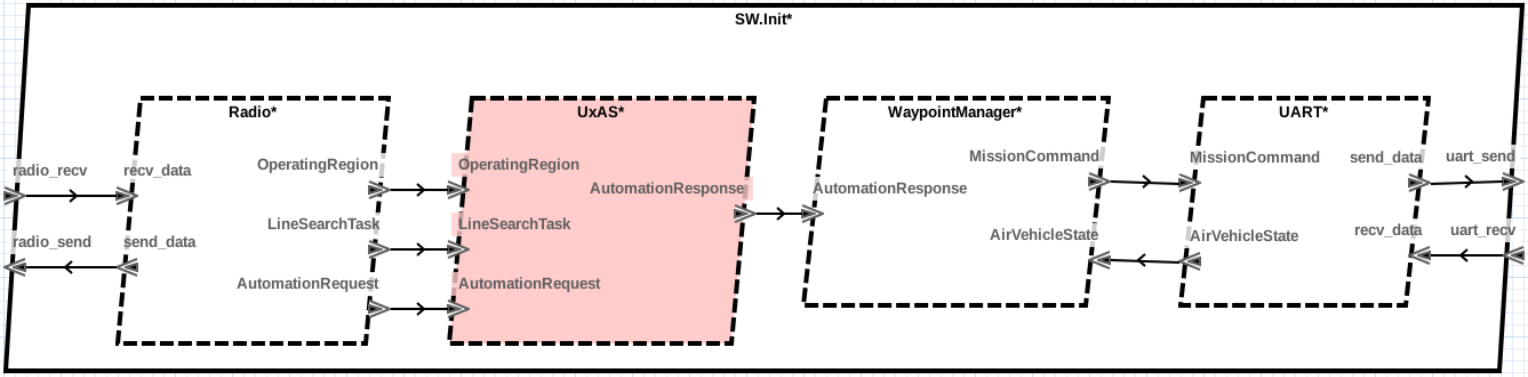
\includegraphics[width=2\columnwidth]{figs/sw-initial.PNG}
	\caption{Initial software architecture.}
	\label{fig:sw-initial}
\end{figure*}

Within the software model, we have formalized some of the high-level requirements as assume-guarantee contracts.
%
We perform a formal analysis with \agr\ to verify that the model satisfies the contracts.
%
For the initial version of our design, the verification passes.
%
Although we are satisfied with the results of the formal verification using AGREE, we have not yet analyzed the design for cyber-vulnerabilities.

In \brfcs, we analyze the model using one (or more) of the integrated cybersecurity analysis tools.
%
As the designers of the system, we reviewed the list of potential vulnerabilities, and then added new requirements to the system model.
%
For example, the vulnerbility analysis noted that UxAS is an open source project, so we marked that component as \texttt{uncontroled} (colored red in \figref{fig:sw-initial}) and added requirements for ensuring that unverified or malicious code (which could potentially be embedded in the component) is not able impact other components.

In total, we added seven cyber requirements from the vulnerability analysis into our model.
%
These include four wellformedness requirements on data, two requirements for monitoring the behavior of the open-source UxAS component, and an attestation requirement for ensuring the integrity of the Ground Station software.
%
Requirements are imported into the model as goals in the assurance case.
%
Because we can build the assurance case at any time during development, we can easily determine for a given snapshot of the model which requirements are not yet supported by evidence.

The intent of the wellformedness requirements is to prevent malformed messages from causing a buffer overrun or code injection attack.
%
In the UAV design, such messages are most likely to originate from a remote source or the uncontrolled UxAS component.
%
By placing filters on the connections upstream of mission-critical components, such attacks could be mitigated.
%
The Filter transform is therefore applied for each wellformedness requirement, inserting filter components on the incoming and outgoing UxAS connections.

The filter code contracts for the four UxAS connections are similar, and check that record values contained in the messages are within appropriate ranges.
%
For example, the Automation Response message filter, which drops messages containing malformed flight plans, is defined as shown in \figref{fig:automation-response-filter}.
%
Although \texttt{Latitude}, \texttt{Longitude} and \texttt{Altitude} are defined as 64-bit floating-point values, the filter only passes messages containing waypoint values between [-90,90], [-180,180], and [0,15000], respectively.

\begin{figure}[h]
	\centering
	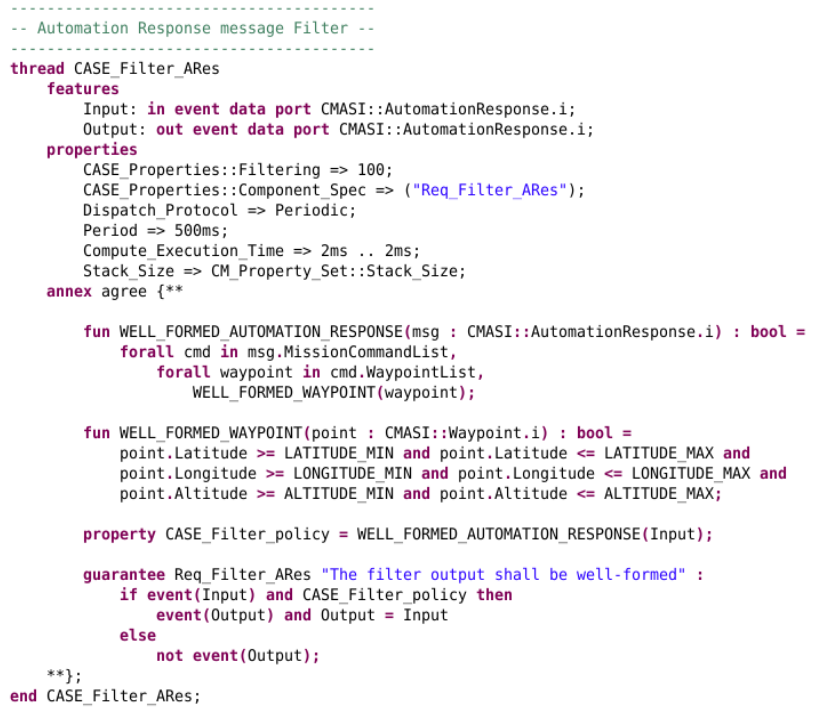
\includegraphics[width=1\columnwidth]{figs/automation-response-filter.png}
	\caption{Automation Response Filter specification.}
	\label{fig:automation-response-filter}
\end{figure}

In addition to monitoring the UxAS output for malformed messages, we must also monitor for suspicious behavior.
%
This requires adding components for detecting that UxAS has crashed, as well as monitoring the correctness of the flight plans it produces.
%
The Monitor transform is applied for this class of mitigation.
%
We add a \textit{response} monitor to send an alert if UxAS does not emit a response within a set amount of time from receiving a request.
%
And we add a \textit{geofence} monitor to ensure that generated flight plans are compliant with the specified keep-in and keep-out zones.
%
The Geofence Monitor is a gated monitor in that it prevents the observed automation response from reaching the Waypoint Manager if the zones are violated.
%
The Geofence Monitor code contract is shown in \figref{fig:geofence-monitor}.

\begin{figure}[h]
	\centering
	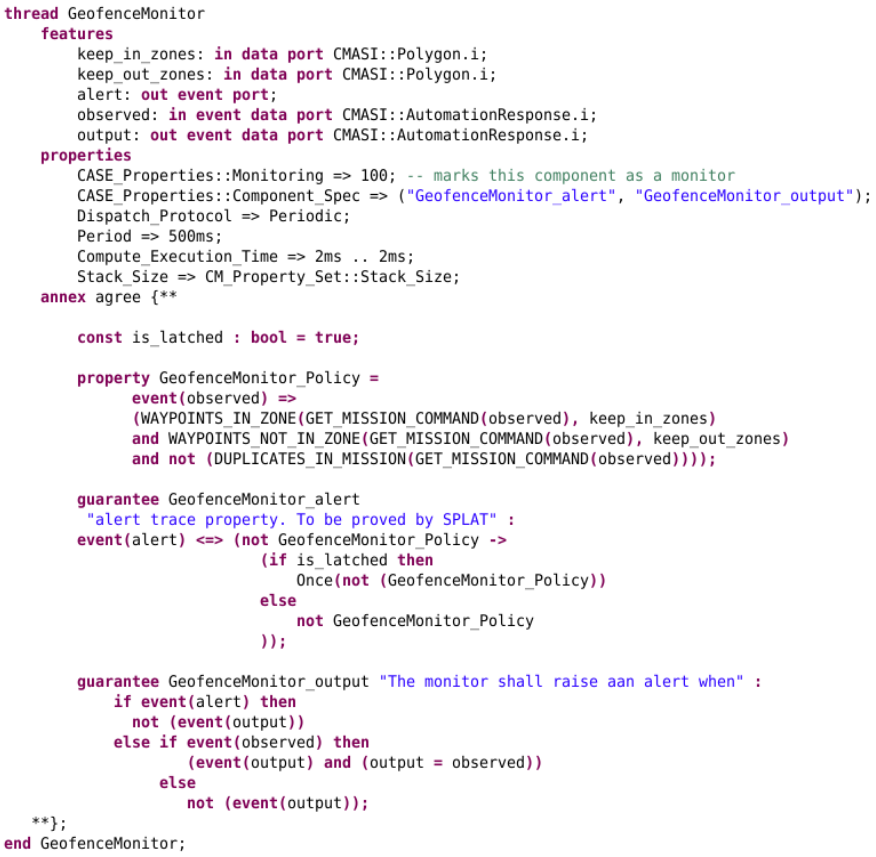
\includegraphics[width=1\columnwidth]{figs/geofence-monitor.png}
	\caption{Geofence Monitor specification.}
	\label{fig:geofence-monitor}
\end{figure}

So far, we have addressed requirements that mitigate vulnerabilities related to malformed messages and malicious behavior \textit{on-board} the UAV.
%
But we also want to protect against a compromised ground station transmitting well-formed, but malicious, commands.
%
The final cyber requirement is mitigated by a transform that adds two components to the UAV software: an Attestation Manager for evaluating remote systems like the Ground Station, and an Attestation Gate for filtering messages from sources that have not been approved by the Attestation Manager.
%
The Attestation Manager \ckml\ implementation is automatically inserted into the application code base by \brfcs.
%
The code contract for the Attestation Gate is completely generated by the transform since its behavior is specific to attestation.

After transforming the model to address the cyber requirements, the software architecture now appears as shown in \figref{fig:hardened-sw}.
%
The shaded components (green) were added by the transform with the exception of the UxAS component (red).

After unit testing the monitors, we formally verify the model with \agr\ to show that all of the component contracts are satisfied.
%
We then run \splt\ to produce provably-correct code.
%
The synthesized code is output to a directory in the build file system with the location specified for each component in the model.
%
The corresponding correctness proof is used in our assurance case as additional evidence that the vulnerability has been properly mitigated.

\begin{figure*}[h]
	\centering
	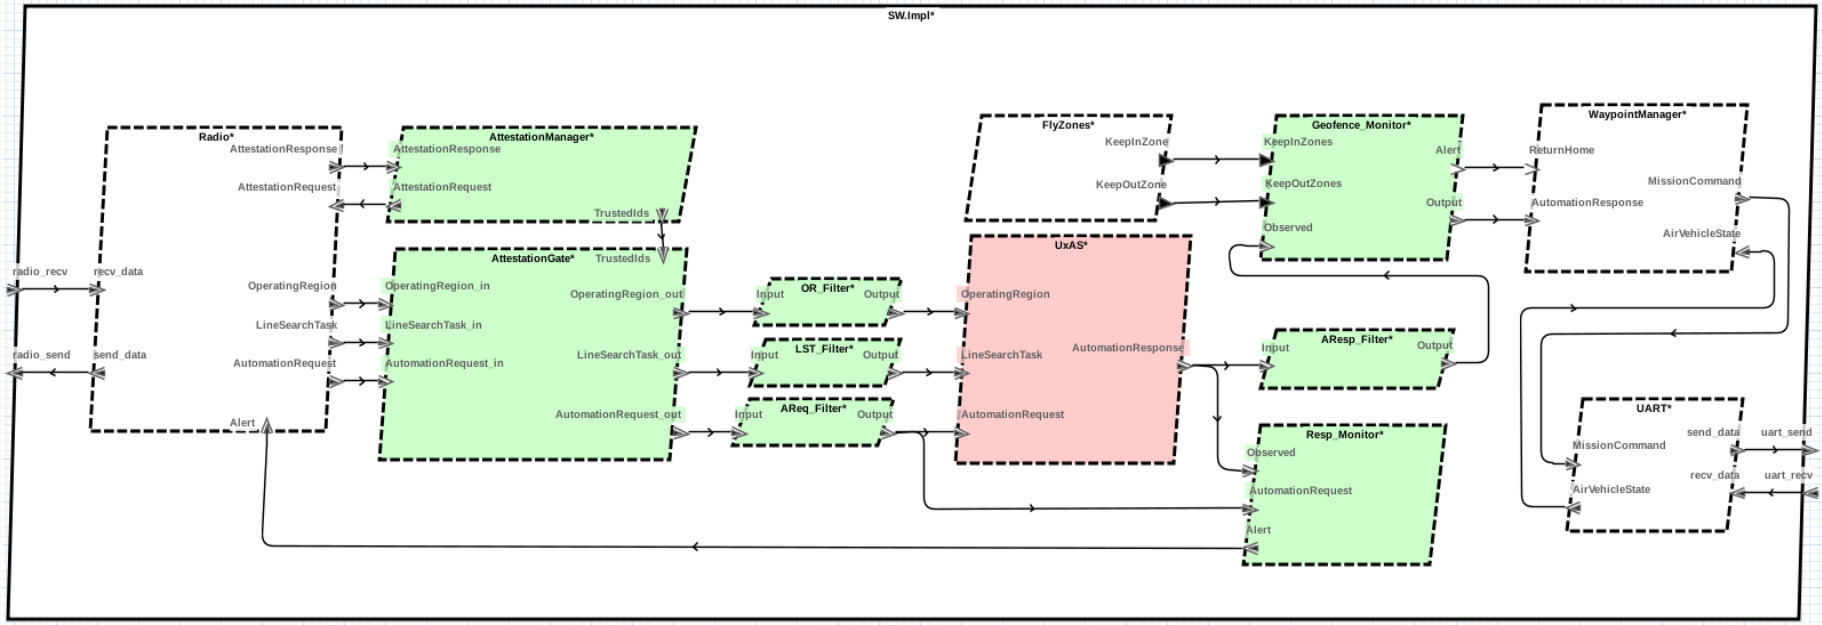
\includegraphics[width=2\columnwidth]{figs/hardened-sw.png}
	\caption{Cyber-resilient software architecture.}
	\label{fig:hardened-sw}
\end{figure*}

Once we have determined that the model is correct and satisfies its cyber requirements, and the software components in the model have been implemented, either by \splt\ or other means, the system can be built and deployed.
%
We run the HAMR tool to generate the component stubs and infrastructure code necessary to enable component communication and execution according to a specified schedule.
%
HAMR then compiles the software to execute on seL4.

The UAV and Ground Station software were deployed on ODROID XU4 hardware, and communicated with each other over ethernet.
%
The AMASE flight simulator, representing the Flight Control Computer was run on a Linux machine and connected to the UAV ODROID via a serial connection.
%
The UxAS implementation on the UAV was modified by adding malicious code that would prevent it from responding to Automation Requests or produce flight plans that would violate the operating region constraints.
%
Some of the Line Search Task messages transmitted from the Ground Station contained malformed messages that would modify the UxAS behavior. In addition, we modified the Ground Station to simulate a breach for our evaluation of the attestation transform.
%
We performed a set of tests on the initial system (\figref{fig:sw-initial}) prior to applying our cyber-resiliency mitigations in order to verify the effectiveness of the malicious code.
A third party evaluator repeated the tests on the hardened system and demonstrated that our mitigation strategy was successful.
%
The following scenarios were exercised:

\paragraph{Infected Ground Station:\/} An application file is modified on the Ground Station, which sends the UAV on a mission-violating trajectory.
%
On the hardened system, messages sent to the UAV were rejected by the Attestation Manager.

\paragraph{Malformed Line Search Task message:\/}
%
The Line Search Task message contained a waypoint with a longitude outside the permitted range to exploit vulnerabilities in the on-board software.
%
The wellformedness filter for Line Search Task messages prevented this message from reaching the UxAS.

\paragraph{UxAS vulnerability exploit:\/} Line Search Tasks with greater than 90 waypoints were transmitted from the Ground Station, triggering a vulnerability that crashes UxAS.
%
When this occurs, UxAS is unable to generate an Automation Response.
%
The response monitor detected and signaled the Ground Station when UxAS failed to respond to the request.

\paragraph{UxAS trojan modifies flight plan:\/} A trojan embedded in UxAS attempts to cause the UAV to fly into a specified keep-out zone by modifying the mission command waypoints in the Automation Response.
%
On the hardened system the Geofence Monitor detected that it was being instructed to fly into a keep-out zone and returned the UAV to Home Base.

%%
% DISSCUSSION
%%

\subsection{Discussion}

The case study demonstrated the viability of writing code contracts and synthesizing implementations from code contracts in a real-world system.
%
It additionally provided insights for improvement.
%
We discovered very early that we needed a mechanism to test contracts.
%
We initially used the synthesis path with a custom test harness for the synthesized code, but this proved to be slow and cumbersome because we had to move back and forth between the OSATE environment and an external test platform.
%
Test contracts are a direct result of our experience, and they obviate the back and forth by integrating test into the modeling and analysis environment.

Writing code contracts for the more complex monitors revealed that although the language is very effective at declarative specifications that define what is being calculated, it is non-intuitive, and sometimes cumbersome, for defining how the computation needs to take place.
%
The primary reason for its unease in describing how computation is performed is that it lacks any type of iterative looping structure for arrays.
%
Instead, it relies on folding and mapping to describe iterative computation which is non-intuitive for many types of array updates.
%
Growing the expressiveness of the language arround arrays is something to investigate in future work.

There are several, practical, low-level concerns that need to be addressed in the high-level model before synthesis takes place that in our process were only discovered after running the actual system on the designated hardware and software.
%
We specifically found it difficult to know the memory bounds for heaps, stacks, and buffers and time bounds for the scheduler \emph{a priori} to code synthesis.
%
As a result, we would have to employ a costly iterative approach to set bounds, synthesize code, and then check if anything failed.
%
Integrating better memory and running time analysis at the modeling level is something to investigate in future work.

\section{Related work}
\label{sec:related-work}

Another model based approach to secure system architectures follows a pattern similar to \brfcs\ with attestation by inserting pre-verified components into the architecture to give certain guarantees \cite{6209212}.
%
In that work, the data connections are annotated with security properties as are the components.
%
A secondary analysis determines if the components meet the security requirements of the data connections, and if not, inserts new security enhancing components in the connection.
%
The insertion algorithm considers time cost when inserting components to preserve worst-case execution times mandated by the system.
%
In the \brfcs\ tool chain there are tools that can analyze the model annotated with security properties and identify where security vulnerabilities may be located, and there are other tools to transform the model to address those vulnerabilities such as those discussed in this paper.

Assume-guarantee reasoning for compositional verification in reactive systems is well-studied \cite{10.1007/978-3-642-28891-3_13, 10.1145/2658982.2527272, 10.1007/978-3-319-17524-9_7}.
%
The first steps toward synthesis of leaf-component contracts determined if leaf-component contracts are realizable \cite{10.1007/978-3-319-17524-9_13, 10.1007/978-3-319-29613-5_7}.
%
These led to algorithms for component synthesis from Lustre models based on realizability \cite{katis2017synthesis, 10.1007/978-3-319-89963-3_10}.
%
The algorithms discover a transition relation that preserves the contract guarantees under all allowed inputs and can be directly transformed into the language intended for the system's implementation.
%
Two such algorithms are implemented in the \agr\ verification engine \cite{jkind}.
%
These synthesis algorithms take in a declarative specification that states \emph{what is to be computed}, and then they have to infer \emph{how to compute it} for the implementation.
%
Code contracts are imperative, by design, so the designer specifies directly how the computation of the high-assurance component takes place thereby avoiding the question of realizability entirely.
%
That said, the test contracts in this paper can be declarative, stating what is to be computed, if desired, and \agr\ can then prove if the code contracts accomplishes that.

Data-flow semantics are well studied \cite{10.1145/41625.41641,97300, 10.1145/1379023.1375674,10.1145/2345141.2248426,10.1007/978-3-540-45212-6_10}.
%
State machine semantics can be added to synchronous data-flow \cite{10.1145/1086228.1086261}.
%
The idea is to translate imperative constructs into equivalent synchronous data flow constructs.
%
The resulting Lustre can then be compiled. The goal is to provide a seamless connection between pure data-flow and pure control design.
%
These approaches are similar to the code contracts in this paper in that they embed imperative computation into the synchronous data-flow semantics of Lustre which are then passed to compilers to render the final target binaries.
%
These compilers however are not verified as is the \ckml\ compiler targeted in this work.

A fully verified compiler has been developed that takes Lustre and compiles it into assembly code, specified and verified in Coq \cite{10.1145/3140587.3062358}.
%
The key is in combining infinite sequences of data-flow models with incremental manipulation of memories akin to an imperative model.
%
CompCert is used on the backend to create the final rendered executable \cite{compcert}.
%
This work is quite similar to ours in providing a verified compilation chain from Lustre.
%
However, there are significant differences: notably, they tackle a more comprehensive subset of Lustre than our work.
%
We have been able to work effectively with a relatively simple core language, \eg, without \emph{clocking} features.
%
This subset aligns with our contract language, and allows us to generate behaviorally equivalent code so we can show that the generated code meets its logical specification.
%
This, in turn, can be used as a leaf-level claim in a system-wide correctness argument conducted by compositional reasoning in \agr.
%
It is important to note that we target a wholistic systems approach to cyber-security that is integrated into the \agr\ reasoning environment whereas the other work targets more specifically a compiler for Lustre.

CoPilot is a domain specific language for writing runtime monitors for hard real-time distributed systems embedded in Haskell and requires working Haskell knowledge to write \cite{10.1007/s11334-013-0223-x}.
%
The language semantics are defined over streams, there is an interpreter for testing the behavior of the runtime monitors, and there are two backend compilers to generate C code.
%
The generated C code is validated by generating random CoPilot programs, generating random input for each program, and checking consensus on output between the interpreter and C programs.
%
Further assurance is accomplished with bounded model checking by showing equivalence between the code from the two compiler backends over a user defined number of steps.
%
Aside from the HOL4 embedding of the code contract semantics and not requiring any HOL4 working knowledge, the work in this paper differs in that it is targeting a fully verified path from the code contract all the way to the binaries leveraging the \ckml\ compiler specifically to provide stronger guarantees on the high assurance components.

As seen in this paper, contracts can be stateful and even higher-order \cite{10.1145/583852.581484}.
%
Verification aware languages compile contracts to runtime monitors \cite{10.1007/978-3-642-28869-2_11}, or omit them when they can statically prove that the code preserves the contract under all possible inputs and executions \cite{10.1145/3158139}.
%
Dafny is a notable verification aware language that provides a contract language, an implementation language, a proof engine to show if an implementation adheres to the contract, and backend compilers for several different target platforms \cite{dafny}.
%
Dafny contracts provide the verification conditions to prove out the implementation code and are not compiled.
%
Compared to the work discussed in this paper, our test contracts are more similar to the Dafny contracts as they are also not compiled and only serve to prove properties of the code contracts.
%
In that regard, the code contracts are the implementation, but unlike Dafny, \ckml\ provide a verified compilation path to binaries.

%%
% CONCLUSION
%%

\section{Conclusion}
\label{sec:conclusion}

Safety critical systems, such as those found in avionics, must be cyber-resilient, i.e. tolerant to cyber-attacks, in the same way that they are fault tolerant.
%
The \brfcs\ environment integrated into OSATE provides systems designers with tools to analyze and address cyber-vulnerabilities in the architectural design of a system modelled using AADL.
%
We have discussed transformations provided by \brfcs\ to insert, create, and synthesize high-assurance components such as filters and monitors to improve the cyber-resiliency of the system design.

A filter enforces invariant properties on data such that data that violate the invariant are not forwarded.
%
A monitor detects and alerts malicious behavior in the system.
%
The actual behavior of such filters, monitors, and other high-assurance components are formally specified by code contracts.
%
A code contract is a subset of the \agr\ language with formal semantics embedded in HOL4 for formal reasoning.
%
A component's code contract states assumptions on the component inputs and provides guarantees that define the component outputs in terms of the component's inputs and current state.
%
The code contract language itself is Turing complete.

Code contracts are validated with unit tests that are verified with the \agr\ verification engine.
%
A unit test in expressed in a test contract in the \agr\ language.
%
A test contract is a stylized contract that strengthens the input assumptions of a code contract to a single input and either weakens or leaves unchanged the code contract output guarantees.
%
\agr\ then proves whether or not the computation expressed in the code contract satisfies the test contract.
%
In this way, a designer is able to test the behavior of the code contract.
%
Once the code contract is tested, the \agr\ verification engine proves whether or not the system, with the added high-assurance components, meets its cyber requirements.

Code contracts are automatically synthesized to \ckml.
%
We discussed the \splt\ synthesis engine that iteratively transforms the code contract defined over streams of data into a state transition function that only considers the current input and state of the component.
%
That state transition function is then rendered in \ckml, and the \ckml\ compiler compiles it to the target binary while also generating the proof of equivalence.

We demonstrated the viability of the approach in real-world industrial design by reporting a case study using the Air Force Research Laboratory's OpenUxAS software.
%
The study required a range of filters, monitors, and other mitigation components to meet cyber-requirements.
%
The case study demonstrated the viability of the approach to address complex message formats and non-trivial cyber-requirements.

The reported case study was carried out by those that created \brfcs\ with its several tools.

Future work is to conduct another case study involving system designers unfamiliar with the \brfcs\ toolchain.
%
We have started such a study with the design of an application using the Collins Common Avionics Architecture System (CAAS)~\cite{caas} on the CH-47F Chinook helicopter program.
%
Early results are encouraging and are revealing ways to expand the expressiveness of the code contract language to make it easier to express iterative computation with arrays.

%%
% FUTURE WORK
%%

\subsubsection*{Future work}

Aside from adding expressiveness to the code contract language, future work is to formally verify every transformation step from the code contract to the final \ckml\ function that is compiled to the target binary.
%
The HOL4 embedding of the code contract semantics we have discussed is the starting point.  The key remaining steps are:
%
\begin{compactitem}
  \item Automatically add state to the code contract to remove $\konst{pre}(-)$ and prove the initial and modified contracts are equivalent for all input streams
  \item Create a step based version of the modified code contract that does not use streams and prove it equivalent to the stream version
  \item Create a pure HOL4 function, suitable to \ckml, from the step version of the code contract and prove it equivalent
\end{compactitem}
%
We have automated in HOL4 the transformation to remove $\konst{pre}(-)$ in the first step in what we call \emph{temporal squashing}.
%
We have additionally written proofs (manually) for every step for a set of example code contracts.
%
From the manual proofs, we have started work on proofs for the first two steps.
%
Since these two steps are universal to all input code contracts their proofs need to be generated just once (as opposed to generating them for every component contract).
%
The proof for the third step must be generated for each input contract.
%
Finally, the entire process needs to be mechanized.
%
Other future work includes lifting the proof results to infinite streams.

\clearpage
\bibliographystyle{plain}
\bibliography{paper}

\end{document}
